 %	Main Document

\documentclass[
	12pt,
	BCOR=5mm,
	DIV=12,
	headinclude=on,
	footinclude=off,
	parskip=half,
	bibliography=totoc,
	listof=entryprefix,
	toc=listof,
	pointlessnumbers,
	plainfootsepline]{scrreprt}

% include configuration file
% !TEX root =  master.tex

% language, font, colors
\usepackage[ngerman]{babel}
\usepackage[utf8]{inputenc}
\usepackage[german=quotes]{csquotes} 	% correct quotes using \enquote{}
\usepackage[T1]{fontenc}
\usepackage{lmodern} % latin modern font, TODO: Arial 12?
\usepackage[onehalfspacing]{setspace}
\usepackage{xcolor}

% hyperlinks
\usepackage[hidelinks=true]{hyperref}

% commands for author and title
\newcommand{\TitelDerArbeit}[1]{\def\DerTitelDerArbeit{#1}\hypersetup{pdftitle={#1}}}
\newcommand{\AutorDerArbeit}[1]{\def\DerAutorDerArbeit{#1}\hypersetup{pdfauthor={#1}}}
\newcommand{\Firma}[1]{\def\DerNameDerFirma{#1}}
\newcommand{\Kurs}[1]{\def\DieKursbezeichnung{#1}}

%\usepackage{microtype}% verbesserter Randausgleich
%\setlength\emergencystretch{1em}
% correct superscripts 
\usepackage{fnpct}

\usepackage{footnote}
\usepackage{rotating} 

% calc 
\usepackage{calc} % Used for extra space below footsepline

% bibliography settings
% author-year-style with footnotes (Chicago)
\usepackage[backend=biber, autocite=footnote, style=authoryear, dashed=false]{biblatex}
\AdaptNoteOpt\footcite\multfootcite
\AdaptNoteOpt\autocite\multautocite

\DefineBibliographyStrings{ngerman}{  % change u.a. to et al. (german only!)
	andothers = {{et\,al\adddot}},
}
% Command to output section title headings
\newcommand{\cvsect}[1]{% The only parameter is the section text
	\vspace{\baselineskip} % Whitespace before the section title
	\colorbox{black}{\textcolor{white}{\MakeUppercase{\textbf{#1}}}}\\% Section title
}

\usepackage{longtable} % Required for tables that span multiple pages
\setlength{\LTpre}{0pt} % Remove default whitespace before longtable
\setlength{\LTpost}{0pt} % Remove default whitespace after longtable

\setlength{\tabcolsep}{0pt} % No spacing between table columns

% Environment to hold a new list of entries
\newenvironment{entrylist}{
	\begin{longtable}[H]{l l}
	}{
	\end{longtable}
}

\newcommand{\entry}[2]{% First argument for the leftmost date(s) text, second is for the entry heading
	\vspace{-0.15cm}
	\parbox[t]{0.33\textwidth}{% 25.0% of the text width of the page
		#1 % Leftmost entry date(s) text
	}%
	&\parbox[t]{0.68\textwidth}{% 75.0% of the text width of the page
		{#2}% Entry heading text
	}\\\\}

\newcounter{barcount}

% Environment to hold a new bar chart
\newenvironment{barchart}[1]{ % The only parameter is the maximum bar width, in cm
	\newcommand{\barwidth}{0.35}
	\newcommand{\barsep}{0.55}
	
	% Command to add a bar to the bar chart
	\newcommand{\baritem}[2]{ % The first argument is the bar label and the second is the percentage the current bar should take up of the total width
		\pgfmathparse{##2}
		\let\perc\pgfmathresult
		
		\pgfmathparse{#1}
		\let\barsize\pgfmathresult
		
		\pgfmathparse{\barsize*##2/5}
		\let\barone\pgfmathresult
		
		\pgfmathparse{(\barwidth*\thebarcount)+(\barsep*\thebarcount)}
		\let\barx\pgfmathresult
		
		\filldraw[fill=none, draw=black!] (0,-\barx) rectangle (5,-\barx-\barwidth);
		\filldraw[fill=black!90, draw=black!90] (0,-\barx) rectangle (\barone,-\barx-\barwidth);
		
		\node [label=180:{\textcolor{black}{##1: ##2/5}}] at (0,-\barx-0.175) {};
		\addtocounter{barcount}{1}
	}
	\begin{tikzpicture}
	\setcounter{barcount}{0}
}{
	\end{tikzpicture}
	\vspace{0.3cm}
}

\usepackage{tikz} % Required for creating the plots
\usetikzlibrary{shapes, backgrounds}
\tikzset{x=1cm, y=1cm} % Default tikz units

%%% Uncomment the following lines to support hard URL breaks in bibliography 
%\apptocmd{\UrlBreaks}{\do\f\do\m}{}{}
%\setcounter{biburllcpenalty}{9000}% Kleinbuchstaben
%\setcounter{biburlucpenalty}{9000}% Großbuchstaben

\setlength{\bibparsep}{\parskip}	% add some space between biblatex entries in the bibliography
\addbibresource{bibliography.bib}	% add file bibliography.bib as biblatex resource

% footnotes (count footnotes over chapters)
\usepackage{chngcntr}
\counterwithout{footnote}{chapter}

% acronyms
\makeatletter
\usepackage[printonlyused]{acronym}
\@ifpackagelater{acronym}{2015/03/20}
  {%
    \renewcommand*{\aclabelfont}[1]{\textbf{\textsf{\acsfont{#1}}}}
  }%
  {%
  }%
\makeatother

% listings
\usepackage{listings}
\renewcommand{\lstlistingname}{Quelltext} 
\renewcommand{\lstlistlistingname}{Quelltextverzeichnis}

%% More configuration for listings is in configlistings.tex %%


% extra packages
\usepackage{graphicx}			% use various graphics formats
\usepackage{subfig}				% sub-figures, e.g. side-by-side pictures
\usepackage[german]{varioref}	% nicer references \vref
\usepackage{caption}			% better captions
\usepackage{booktabs}			% nicer tabs
\usepackage{array}

% algorithms
\usepackage{algorithm}
\usepackage{algpseudocode}
\renewcommand{\listalgorithmname}{Algorithmenverzeichnis}
\floatname{algorithm}{Algorithmus}

% page header/footer
\RequirePackage[automark,headsepline,footsepline]{scrpage2}
\pagestyle{scrheadings}
\renewcommand*{\pnumfont}{\upshape\sffamily}
\renewcommand*{\headfont}{\upshape\sffamily}
\renewcommand*{\footfont}{\upshape\sffamily}
\renewcommand{\chaptermarkformat}{}
\RedeclareSectionCommand[beforeskip=0pt]{chapter}
\clearscrheadfoot

\ifoot[\rule{0pt}{\ht\strutbox+\dp\strutbox}DHBW Mannheim]{\rule{0pt}{\ht\strutbox+\dp\strutbox}DHBW Mannheim}
\ofoot[\rule{0pt}{\ht\strutbox+\dp\strutbox}\pagemark]{\rule{0pt}{\ht\strutbox+\dp\strutbox}\pagemark}

\ohead{\headmark}


\begin{document}

% set some information (title, author, ...)
\TitelDerArbeit{Entwurf und Implementierung eines Kinoreservierungssystems}
\AutorDerArbeit{Sascha Görnert, Rene Fischer, Gerrit Pollkläsener, Erik Jansky, Niko Lockenvitz}
\Firma{DER Touristik GmbH, Technische Universität Kaiserslautern, SAP SE}
\Kurs{WWI 17 SE B}

\begin{titlepage}

\begin{minipage}{\textwidth}
	\vspace{-2cm}
	\noindent
	
\includegraphics[height=0.1\linewidth]{img/logos/der}
	\hfill
	
\includegraphics[height=0.1\linewidth]{img/logos/tukl}
	\hfill
	
\includegraphics[height=0.1\linewidth]{img/logos/sap}
	\hfill
	
\includegraphics[height=0.1\linewidth]{img/logos/dhbw}
\end{minipage}

\vspace{1em}
\sffamily

\begin{center}
	\textsf{\large{}Duale Hochschule Baden-Württemberg\\[1.5mm] Mannheim}\\[2em]
	\textsf{\textbf{\Large{}Seminararbeit}}\\[3mm]
	\textsf{\textbf{\DerTitelDerArbeit}}\\[1.5cm]
	\textsf{\textbf{\Large{}Studiengang Wirtschaftsinformatik}\\[3mm] \textsf{Studienrichtung Software Engineering}}
	
	\vspace{3em}
	\vfill

	\begin{minipage}{\textwidth}
	
		\begin{tabbing}
			Bearbeitungszeitraum: \hspace{0.85cm}\=\kill
			Verfasser: \> Sascha Görnert, 2716910 \\
			\> DER Touristik GmbH \\
			\> \\
			\> Rene Fischer, 8703049 \\
			\> Technische Universität Kaiserslautern \\
			\> \\
			\> Gerrit Pollkläsener, 1930724 \\
			\> SAP SE \\
			\> \\
			\> Erik Jansky, 5980253 \\
			\> SAP SE \\
			\> \\
			\> Niko Lockenvitz, 1308674 \\
			\> SAP SE \\
			\> \\[1.5mm]
			Kurs: \> \DieKursbezeichnung \\[1.5mm]
			Bearbeitungszeitraum: \> 19.11.2018 -- 12.02.2019
	\end{tabbing}

	\end{minipage}

\end{center}

\end{titlepage}

\pagenumbering{roman}
\normalfont

% abstract
\chapter*{Kurzfassung}
\begingroup
\begin{table}[h!]
\setlength\tabcolsep{0pt}
\begin{tabular}{p{3.7cm}p{11.7cm}}
Titel & \DerTitelDerArbeit \\
Verfasser: & \DerAutorDerArbeit \\
Kurs: & \DieKursbezeichnung \\
\end{tabular}
\end{table}
\endgroup

Zusammenfassung der Arbeit

% table of contents
\tableofcontents

% figures
\listoffigures

% tables
%\listoftables

% listings (source code)
\lstlistoflistings

% acronyms
\clearpage
\chapter*{Abkürzungsverzeichnis}
\addcontentsline{toc}{chapter}{Abkürzungsverzeichnis}

\begin{acronym}[A23456789012] % longest acronym for correct indentation
	\acro{A23456789012}{This is just for indentation}

	\acro{AJAX}{Asynchronous JavaScript and XML}
	\acro{API}{Application Programming Interface}
	\acro{CRUD}{CREATE, READ, UPDATE, DELETE}
	\acro{CSS}{Cascading Style Sheets}
	\acro{DAO}{Data Access Object}
	\acro{DBMS}{Datenbankmanagementsystem}
	\acro{DOM}{Document Object Model}
	\acro{DTO}{Data Transfer Object}
	\acro{ER-Modell}{Entity-Relationship-Modell}
	\acro{HTML}{Hypertext Markup Language}
	\acro{HTTP}{Hypertext Transfer Protocol}
	\acro{HTTPS}{Hypertext Transfer Protocol Secure}
	\acro{IDE}{Integrated Development Environment}
	\acro{JPA}{Java Persistence API}
	\acro{JPQL}{Java Persistence Query Language}
	\acro{JSON}{JavaScript Object Notation}
	\acro{ORM}{Objektrelationaler Mapper}
	\acrodefplural{ORM}{Objectrelationale Mapper}
	\acro{POJO}{Plain Old Java Object}
	\acro{REST}{Representational State Transfer}
	\acro{SQL}{Structured Query Language}
	\acro{URI}{Uniform Resource Identifier}
	\acro{URL}{Uniform Resource Locator}
\end{acronym}

\ohead{Acronyms}

%--------------------------------
% Content
%--------------------------------
\clearpage
\ihead{\chaptername~\thechapter}
\ohead{\headmark}
\pagenumbering{arabic}

% one file for each chapter
% !TEX root =  master.tex
\chapter{Einleitung}

Diese Seminararbeit beschreibt das im Umfang des Moduls Fallstudie entwickelte Kinoreservierungssystem der Gruppe um Sascha Görnert, Rene Fischer, Erik Jansky, Niko Lockenvitz und Gerrit Pollkläsener.
Zielsetzung des zu entwickelten Systems ist es, einem Nutzer die Online-Buchung eines (oder mehrerer) Kinotickets zu ermöglichen.
Eine genauere Erläuterung der eigens gesetzten Ziele sowie eine Betrachtung, inwiefern diese erreicht wurden, findet in Kapitel \vref{sec:ziele} statt.
In den folgenden Abschnitten werden die durchlaufenen Entwicklungsschritte, einschließlich Planungsphase, Umsetzung und Reflexion erläutert und spezifiziert.

% !TEX root =  master.tex
\chapter{Analyse}
\chaptermulitpleauthor{\authorSG}{\authorGP, \authorRF, \authorEJ}

% !TEX root =  master.tex
\section{Personas}

In der Analysephase wurden folgende Personas erstellt:
\begin{enumerate}
\item Johnny Cash
\item Leon Schweickert
\item Florentina Kastenkette
\item Familie Mandick
\item Oma Gertrud
\end{enumerate}
% !TEX root =  master.tex
\section{User-Stories}

Mit der großen Spannbreite an Personas gibt es auch zahlreiche, teils sich stark unterscheidende Anforderungen an das Kinobuchungssystem.
Im folgenden Abschnitt werden diese Wünsche der Personas aufgezählt und gruppiert.

\subsection{Übersicht / Filmauswahl}
Zuerst werden die Anforderungen an eine Übersicht über das aktuelle Filmprogramm geschildert.

\cvsect{Florentina Kastenkette}
Als Florentina Kastenkette interessiere ich mich primär nur für eine schnelle Übersicht über die neuesten und beliebtesten Filme.

\cvsect{Leon Schweickert}
Für mich als Leon Schweickert ist eine ausführliche Auflistung aller Filme geeigneter.
Hier könnte ich mich über alle Filme genauer informieren, mir Besetzung oder eine Vorschau ansehen und sogar eine Kurzbeschreibung des Films durchlesen.
Als Leon Schweickert würde würde ich mich eventuell sogar für einen Newsletter mit dem Kinoprogramm interessieren, den ich einfach per Mail erhalte.

\cvsect{Familie Mandick}
Als Familie Mandick legen wir einen größeren Wert darauf, das oftmals große Filmprogramm nach Genre oder \acs{FSK}-Bewertung filtern zu können.
Hierdurch ließen sich für die ganze Familie geeignete Filme schnell finden, was auch durch eine Suchfunktion erreicht werden könnte.
Dies würde uns trotz unserer spontanen Natur einen kurzfristigen Kinobesuch erleichtern.

\cvsect{Oma Gertrud}
Als Oma Gertrud ist all das jedoch kaum relevant, da ich mit einem dieser Computer kaum zurecht komme, was ich ja auch nicht lernen muss, da sich dieses Internet eh nicht lange halten wird.
Für mich wäre eine ausgedruckte Version der Übersicht in Form einer Zeitungsanzeige oder eines Flyers wesentlich zugänglicher.

\subsection{Auswahl einer Vorstellung}
Nach der Auswahl eines Films folgt die Wahl einer Vorstellung (Zeit und Datum).

\cvsect{Johnny Cash}
Hier ist es für mich als Johnny Cash sehr wichtig, eine klare Übersicht über die nächsten Vorstellungen zu bekommen, um so schnell wie möglich den passenden Termin für die Kunden zu finden.
Hierbei sind für mich vor allem die zeitnahen Vorstellungen relevant, da die meisten Kunden am Schalter direkt Tickets für die Vorstellungen am selben Abend kaufen.
Bei Fragen nach zukünftigen Filmvorstellungen würde ich zwar gern nach solchen Filmen filtern können, an sich treten solche Fälle jedoch wesentlich seltener auf.

\cvsect{Leon Schweickert}
Auch für mich als Leon Schweickert spielt Geschwindigkeit eine große Rolle: Ich hätte am liebsten schon bei der Übersicht die Vorstellungszeiten am aktuellen Tag, damit ich mir einen Klick sparen kann.

\cvsect{Florentina Kastenkette}
Eine eigene Seite zur Vorstellungsauswahl wird jedoch von mir als Florentina Kastenkette bevorzugt, da ich mit meinen Freundinnen am Telefon gemeinsam aushandeln muss, wann alle Zeit haben, und dabei eine große Übersicht echt praktisch wäre.
Außerdem möchte ich schnell erkennen oder filtern können, welche Vorstellungen in 2D bzw. 3D sind, und ob die Filme in deutscher Sprache oder in ihrer Originalfassung aufgeführt werden.

\cvsect{Oma Gertrud}
Als Oma Gertrud möchte ich lieber im Kino anrufen und mir eine Vorstellungsauswahl von einem Mitarbeiter ansagen und anschließend einen Platz auf meinen Namen reservieren lassen.

\subsection{Sitzplatzauswahl}
\cvsect{Florentina Kastenkette}
Bei der Platzauswahl ist es mir als Florentina Kastenkette wichtig, mehrere Plätze mit unterschiedlichen Ermäßigungsstufen auswählen zu können, da ich neben meinen Freundinnen auch gern meine kleine Schwester mit ins Kino nehme.

\cvsect{Leon Schweickert}
Als Leon hingegen erwarte ich eine hübsche grafische Platzauswahl, bei der man auf einen Blick zwischen belegten und unbelegten Plätzen unterscheiden kann.

\cvsect{Johnny Cash}
Für mich als Kassierer Johnny Cash ist es wichtig, dass die von mir getätigten Reservierungen und Buchungen vor denen der Online-Nutzer Vorrang haben, damit mir keine Plätze beim Bedienen der Kunden vor Ort \enquote{weggeschnappt} werden.
Dies würde einerseits meinen täglichen Ablauf vor Ort erschweren und mich andererseits unprofessionell wirken lassen.

\subsection{Bezahlung}
\cvsect{Oma Gertrud}
Ich als Oma Gertrud möchte meine Tickets nur reservieren und später im Kino bar bezahlen, da ich selbst nicht weiß, wie man Geld mit dem Computer verschicken könnte.

\cvsect{Florentina Kastenkette}
Auch als Florentina bezahle ich lieber vor Ort, dies liegt jedoch daran, dass ich überall mit meiner EC-Karte bezahle, damit ich meine Kosten immer im Blick behalten kann und es meistens schneller geht als mein Bargeld herauszukramen.
Falls ich jedoch mal online bezahle, möchte ich mich aber nicht mit einem Konto anmelden müssen, da ich \enquote{nur} sozialen Netzwerken meine Nutzerdaten anvertraue.

\cvsect{Leon Schweickert}
Ganz anders geht es mir hier als Leon: Ich bevorzuge es, online per PayPal zu bezahlen und möchte am liebsten bei meinem Nutzerkonto ein bevorzugtes Zahlungsmittel hinterlegen können, um dies nicht bei jeder Buchung erneut eintragen zu müssen.

\cvsect{Johnny Cash}
Als Johnny Cash ist es mir an der Kasse wichtig, eine möglichst große Anzahl an Bezahlungsmitteln anbieten zu können, um den Bezahlvorgang so unproblematisch wie möglich gestalten zu können.
Außerdem möchte ich keine Gesamtpreise selbst errechnen müssen, sondern schnell den Preis für bereits reservierte Tickets herausfinden können, ohne groß danach suchen zu müssen.

\subsection{Bestätigung}
\cvsect{Leon Schweickert}
Neben einer allgemeinen Bestätigung auf der Webseite, dass die Bezahlung, Buchung oder Reservierung erfolgreich gewesen ist, möchte ich als Leon nach meiner Buchung das Ticket direkt auf meinem Handy zur Verfügung stehen haben.

Ob das per App oder Mailversand passiert, ist mir dabei eher unwichtig, ich möchte bloß \enquote{unnötigen Papierkram} umgehen.

\cvsect{Florentina Kastenkette}
Da ich als Florentina sehr aktiv in sozialen Netzwerken unterwegs ist, wäre es mir wünschenswert, eine \enquote{Teilen}-Funktionalität auf der Bestätigungsseite zu haben, damit ich direkt online mit all meinen Freunden teilen kann, wann und wo der Kinobesuch stattfindet.
Dies würde mir ein lästiges erneutes Eintippen der Daten ersparen.

\subsection{Reservierungsbearbeitung}
\cvsect{Familie Mandick}
Die Möglichkeit, getätigte Reservierungen online oder per Anruf spontan kündigen zu können, spielt für unsere Familie Mandick eine große Rolle.
Hiermit können wir sicher gehen, dass wir nicht unnötig Geld für die Tickets verschwenden, wenn vielleicht wieder etwas dazwischen kommt.

\cvsect{Leon Schweickert}
Als Leon möchte ich meine Reservierungen oder gekauften Tickets per Knopfdruck in meinen (mobilen) Kalender übertragen können, wobei ich gern auch noch eine eigene Notiz anhängen können würde.

\subsection{Im Kino}
\cvsect{ Oma Gertrud}
Ein ausgedrucktes Ticket an der Kasse zu erhalten ist für mich als Oma Gertrud sehr wichtig, da ich gern \enquote{etwas Festes in der Hand} habe und nicht nur \enquote{so eine komische Würfelgrafik}.

\cvsect{Johnny Cash}
Als Johnny ist es mir dementsprechend wichtig, online oder am Telefon reservierte Tickets an der Kasse schnell ausdrucken zu können.

\cvsect{Familie Mandick \& Leon Schweickert}
Die Familie Mandick und Leon Schweickert wollen den Schritt an der Kasse lieber überspringen.
Als Leon bevorzuge ich es, die gesparte Zeit zum Popcorn-Kauf aufzuwenden, während wir, die Eltern Mandick, bloß ein Rumgequengele unserer Kinder in der Warteschlange verhindern wollen
Außerdem wäre ein schneller Weg zum Kinosaal für uns sehr nützlich, wenn wir mal wieder \enquote{punktgenau} zum Filmstart im Kino ankommen und uns beeilen müssen, um nicht den Filmstart zu verpassen.

\cvsect{Florentina Kastenkette \& Leon Schweickert}
Als einer der beiden eher jungen Nutzer Florentina oder Leon wäre es außerdem praktisch, wenn ich nicht jedes Mal im Kino den Studentenausweis vorzeigen müsste, sondern ich diesen entweder bei der Buchung angeben oder im Profil hinterlegen könnte, falls man ihn mal vergisst.

\subsection{Sonstiges}
Die sonstigen Wünsche beziehen sich hauptsächlich auf häufige Besucher und Webseiten-Nutzer wie Leon.

Das Abspeichern von Filterpräferenzen, eine Einsicht der eigenen Kinohistorie und -statistik oder das Erstellen von Bewertungen und Kommentaren für die besuchten Filme wären Features, die die Webseite interaktiv für den Anwender gestalten würden.

Außerdem wäre es für mich als Leon nützlich, von Rabattaktionen oder Bonusprogrammen profitieren zu können, da ich so oder so viel Zeit im Kino verbringe.

% !TEX root =  master.tex
\section{User-Journey}

% !TEX root =  master.tex
\section{Ablauf im Kino}


% !TEX root =  master.tex
\chapter{Entwurf}
\label{c:entwurf}

% !TEX root =  master.tex
\section{Klassendiagramm}
\label{sec:Klassendiagramm}
\multipleauthorsection{\authorSG}{\authorNL}

Das Klassendiagramm wurde im Verlauf des Projekts mehrfach angepasst.
Der erste Entwurf befindet sich in Anhang \vref{fig:anhang_klassendiagramm01}.
Die aktuelle Version ist in Anhang \vref{fig:anhang_klassendiagramm02} zu finden.

% !TEX root =  master.tex
\section{Sequenzdiagramm}
\label{sec:sequenzdiagram}
\authorsection{\authorSG}

Im Anhang \vref{fig:Anhang_seq_reservieren} befindet sich ein Sequenzdiagramm des Reservierungsvorganges.

Im folgenden werden die einzelnen Schritte kurz erläutert. 

Nachdem der Benutzer die gewünschten Sitzplätze ausgewählt hat, drückt er im Front-End auf den Button Reservieren. 
Das Front-End erstellt darauf hin ein \acs{JSON}, mit den Informationen der gewünschten Sitzplätze (siehe  \vref{lst:json_book}). 
Vor dem \acs{JSON} wird noch ein Formparameter book angeschlossen, um eine genauere Identifizierung in der \acs{REST}-Schnittstelle \jinline|reservation/book| zu realisieren. 

Das Front-End ruft über eine \acs{AJAX}-Call den Webserver mit der \acs{URI}  \url{http://localhost:8080/cinemasystem-system/reservation/book} auf und übergibt das \acs{JSON}. 
Diese Ressource ruft ihren eigenen Service auf. 
Dieser ruf den Webserver für die Datenschicht über die \acs{URI} \url{http://localhost:8080/cinemasystem-data/reservation/book} auf und übergibt das \acs{JSON}. 
Hier wird das \acs{JSON} in ein \acs{DTO} mittels eines \acs{JSON}-Converters konvertiert.
Da aus dem Front-End lediglich die  Vorstellungs-ID kommt, müssen die Informationen der Vorstellung aus der Datenbank geholt werden. \\
Hier wird die Methode \jinline|find(String id)| im \jinline|ShowService|, der ebenfalls in der Ressource implementiert ist, aufgerufen. 
Diese greift auf die Datenbank zu und holt die Informationen der Vorstellung ab und wandelt es anschließend in ein Show-\acs{DTO} um. 

%Anschließend kann eine Verifizierung erfolgen, ob überhaupt eine Reservierung derzeit möglich ist. 
%Ein möglicher Ausschlussgrund könnte sein, dass zwischen Beginn der ausgewählten Vorstellung weniger als 30 Minuten liegen. \\
%Ist diese erfolgreich gewesen, wird überprüft, ob es bereits den Kunden in der Datenbank gibt. 
%Dies wird durch die vom Front-End übermittelte E-Mail-Adresse des aktuellen Benutzers ermittelt. 
%Somit kann später der Reservierung und somit den Tickets eindeutig der Kunde zugewiesen werden. \\

Anschließend erfolgen verschiedene Verifizierungen, ob das Anlagen der Reservierung möglich ist.
Ausschlussgründe könnten sein:
\begin{enumerate}
	\item Zwischen Vorstellung und aktueller Uhrzeit liegen weniger als 30 Minuten.
	\item Der ausgewählte Sitzplatz ist schon von einem anderen Benutzer blockiert.
	\item Der ausgewählte Sitzplatz ist bereits vergeben.
\end{enumerate}
War die Reservierung erfolgreich, wird das Ergebnis an den \jinline|ReservationService| des Webserver System im \acs{JSON} zurück übermittelt.
Ggf. kann es hier noch zu weiteren Berechnungen kommen, weshalb das \acs{JSON} in ein Reservation\acs{DTO} umgewandelt wird.

Ist die Methode \jinline|postTickets| abgeschlossen, wird das Ergebnis in ein \acs{JSON} umgewandelt und an das Front-End gesendet, welches dem Benutzer die Reservierung als QR-Code darstellt (siehe Kapitel \vref{fig:vorstellung04}).

Eine nähere Beschreibung der Herausforderungen für das Reservieren und den Lösungsansätzen befindet sich in Kapitel \vref{ssec:herausforderung_reservieren} und Kapitel \vref{ssec:loesung_reservieren}.

% !TEX root =  master.tex
\section{Authentifzierung}

Kunden sollen die Möglichkeit haben, sich zu registrieren.
Dabei setzen sie ein Passwort, welches im Anschluss gemeinsam mit der E-Mail-Adresse zur sicheren Authentifizierung dient.

Das Passwort wird dabei nicht im Klartext gespeichert, sondern in Form eines Hash\-wertes. % TODO: Details Hash + Quelle
Bei der Berechnung des Hash\-wertes wird ein benutzer\-spezifischer Salt mit dem Passwort verknüpft, um die Passwörter gegen Angriffe mit \enquote{Rainbow Tables} abzusichern. % TODO: Erläuterung + Quelle
Der Hash aus Salt und Passwort wird in der Datenbank gespeichert, sodass ein Ausschnitt der Datenbank in vereinfachter Form wie folgt aussehen könnte:

\setlength{\tabcolsep}{6pt}
\begin{tabular}{|l|l|l|}
	\hline
	email & salt & hashSHA1 \\
	\hline
	max@muster.de & 1952e9 & 3b9c4352194e71abfc3931f6634ef6355018149b \\
	\hline
	erika@musterfrau.eu & d4aeff & f8b2f89758a31e17228233b5bd26b7267aa92ea8 \\
	\hline
\end{tabular}

In beiden Fällen ist das Klartextpasswort \enquote{geheim}.
Durch den Salt ist dies aber nicht direkt erkennbar.

Wenn sich nun ein Benutzer versucht anzumelden, gibt er das Passwort an.
In der Verarbeitungsschicht muss dann zum betreffenden Nutzer der Salt herausgesucht werden, mit dem eingegebenen Passwort verknüpft und anschließend gehasht werden.
Stimmt dieser Hash mit dem aus der Datenbank überein, so war das Passwort korrekt und der Nutzer konnte seine Identität erfolgreich bestätigen.

Wenn sich ein Kunde mit seinem Benutzerkonto erfolgreich anmeldet, wird eine \textit{Session\-ID} erzeugt.
Diese wird sowohl in der Datenbank und als auch in Form eines Cookies im Webbrowser des Benutzers gespeichert, damit im folgenden Verlauf einerseits die Authentifizierung gewährleistet bleibt und andererseits das Passwort nicht mehr benutzt werden muss. % TODO: Quelle

Jeder benutzer\-spezifische Aufruf der \acs{API} muss dann eine eindeutige Identifikation des Benutzers, z.B. die E-Mail-Adresse und die \textit{SessionID} des Benutzers enthalten, damit in der Verarbeitungsschicht sichergestellt werden kann, dass die auszuführende Aktion auch autorisiert ist. % TODO: Erläuterung am Beispiel

% !TEX root =  master.tex
\section{Sitzplatzauswahl und Blockierungen}
\authorsection{\authorNL}

Beim Reservierungsvorgang ist es essentiell, dass ein Sitzplatz nicht mehrfach reserviert wird.

Hier ein einfaches Beispiel:
Benutzer A besucht die Seite, wählt einen Film und eine Vorstellung aus.
Die Saalübersicht wird geladen, wobei Sitzplätze, die bereits reserviert sind, optisch hervorgehoben sind und nicht mehr ausgewählt werden können.
Etwa zur gleichen Zeit besucht Benutzer B die Seite.
Er wählt die selbe Vorstellung, sieht die gleiche Saalübersicht und wählt einen Platz aus: Reihe 4, Platz 2.
Benutzer B folgt daraufhin den weiteren Schritten, bezahlt seinen Sitzplatz und erhält eine Bestätigung, dass Reihe 4, Platz 2 erfolgreich von ihm gebucht wurde.
Auch Benutzer A hat Reihe 4, Platz 2 ausgewählt.
Zu dem Zeitpunkt als Benutzer A den Saalplan geladen hat, war die Reservierung von Benutzer B noch nicht abgeschlossen, sodass der Platz frei war.
Auch Benutzer A möchte nun das Ticket bezahlen, muss aber eine Fehlermeldung erhalten, damit das Ticket für Reihe 4, Platz 2 nicht doppelt verkauft wird.

Spätestens bei der verbindlichen Reservierung und der normalerweise folgenden Bestätigung muss eine Fehlermeldung erscheinen, wenn der Platz bereits belegt ist.
Im Idealfall wird der Nutzer aber schon früher benachrichtigt, wenn er einen Platz ausgewählt hat, der in der Zwischenzeit von einem anderen Benutzer reserviert wurde.

Der Fall, dass ein Platz durch einen anderen Benutzer reserviert wird, ist mit gewisser Wahrscheinlichkeit vorhersehbar.
Wählt ein Benutzer im Saalplan ein paar Plätze aus, so wird er vermutlich in den nächsten paar Minuten mit der Bezahlung fortfahren und die Plätze für sich reservieren.
In dem Moment, wo ein Benutzer einen Sitzplatz also nur auswählt, kann diese Information bereits in der Datenbank gespeichert werden.
Der Sitzplatz wird für diesen Benutzer zwar nicht reserviert, aber für einen kurzen Zeitraum vorgemerkt.
Will nun jemand einen Platz auf dem Saalplan auswählen, teilt er dies über die \acs{API} dem Back-End mit.
Nun gibt es mehrere mögliche Ergebnisse:
\begin{enumerate}
\item Der ausgewählte Sitzplatz ist bereits reserviert.
\item Der ausgewählte Sitzplatz ist bereits für einen anderen Benutzer vorgemerkt, könnte also in einigen Minuten wieder frei werden.
\item Der Sitzplatz ist weder reserviert, noch vorgemerkt.
Er wurde nun erfolgreich für den aktuellen Benutzer vorgemerkt.
\end{enumerate}

Dies kann nun dazu führen, dass ein Benutzer einen freien Saalplan angezeigt bekommt und beim Anklicken eines Platzes dieser nun nicht mehr als \enquote{frei}, sondern als \enquote{durch einen anderen Nutzer belegt} angezeigt wird.

Die zu der Reservierung zugehörigen Operationen auf der Datenbank müssen atomar ausgeführt werden, sodass die Reservierung entweder erfolgreich war oder eine Fehlermeldung den Benutzer informiert, dass die Reservierung fehlgeschlagen ist.

Alle Sicherheitsprüfungen müssen im Back-End ausgeführt werden.
Natürlich können auch einzelne Prüfungen im Front-End implementiert werden, diese helfen allerdings nur einem normalen Benutzer den Vorgang zu erleichtern.
Eine Absicherung bieten derartige Prüfung im Front-End nicht, da der clientseitig ausgeführte Quellcode logischerweise vom Client verändert werden kann und jeder Angreifer eine manipulierte Anfrage mit selbst gewählten Parametern an die \acs{API} schicken kann.

% backend content
\chapter{Back-End}
\chapterauthor{Sascha Görnert}
\section{Technologien}
\label{sec:technologien}

Für das hier erstellte Kinoreservierungsprogramm wurde die Verwendung von Java\footnote{\url{https://java.com/de/download/} -- Version 8.0.141 verwendet} für das Back-End vorgegeben. 

Als Java-\acs{IDE} kommt Eclipse\footnote{\url{https://www.eclipse.org/} -- Version: Photon Release (4.8.0)} zum Einsatz, da es aus vorangegangenen Vorlesungen bekannt ist.
Für die Kommunikation zwischen den einzelnen Schichten der Drei-Schichten-Architektur kommen \acs{REST}ful-Webservices in Verbindung mit Jersey\footnote{\url{https://jersey.github.io/} -- Version 1.19.4} sowie \acp{DTO} zum Einsatz (Kapitel \vref{sec:dto}), die zwischen den einzelnen Schichten transferiert werden.

Um eine Datenhaltung und den Austausch von Informationen zu gewährleisten, wurde sich in dieser Arbeit für eine Postgres Datenbank entschieden.
Der Zugriff auf die Datenbank erfolgt mittels der \ac{JPA} in Verbindung mit EclipseLink (Kapitel \vref{ssec:jpa}).
% !TEX root =  master.tex
\section{Konzept}
\label{sec:konzept}
\authorsection{\authorSG}
In diesem Projekt soll die Drei-Schichten-Architektur eingesetzt werden.
Sie dient dazu, die einzelnen Schichten (Datenhaltung, Fachkonzept und Benutzeroberfläche) zu separieren, sodass in zukünftigen Schritten ein Austausch der genutzten Benutzeroberfläche oder Datenbank möglich ist. 

Wie zuvor in Kapitel \vref{sec:technologien} beschrieben, finden in diesem Projekt \acs{REST}ful Webservices Anwendung.
Da Webservices in der Realität u.a. aus Performance-Gründen auf unterschiedlichen Servern ausgeführt werden, wurde dies hier ebenfalls umgesetzt.
Zum Einsatz kommt eine System- und Data-Webservice.
Wie in Abbildung \vref{fig:konzept_backend} dargestellt ist, greift die Benutzeroberfläche niemals direkt auf die Datenhaltungsschicht zu.
Dies wird realisiert, indem das Front-End auf die bereitgestellten Webservices von System in der Fachkonzeptschicht zugreift. 
Diese wiederum greifen dann auf die Webservices der Datenhaltungsschicht zu.

\begin{figure}[ht]
	\centering
	
\includegraphics[width=0.7\textwidth]{img/backend/rest}
	\captionsetup{format=hang}
	\caption{Konzept des Back-Ends}
	\small Quelle: eigene Darstellung mittels \url{https://draw.io/}
	\label{fig:konzept_backend}
	\end{figure}

Für dieses Projekt werden drei Hauptklassen in Java verwendet: \textit{Shared}, \textit{System} und \textit{Data}. 
In der Klasse \textit{Shared} befinden sich alle gemeinsam genutzten Klassen wie z.B. u.a. die verwendeten \acp{DTO}, Konvertierungs-Methoden, ausgelagerten Überprüfungen und der \acs{JSON}-Converter, der das \acs{DTO} in ein \acs{JSON} umwandelt. 

Die System-Ressource stellt dem Front-End mehrere \acs{REST}-Schnittstellen zur Verfügung.
Nachdem die Ressource über eine \acs{URI} \url{http://localhost:8080/cinema-system/show/1} aufgerufen wurde, ruft diese z.B. die Methode \jinline |getMovieById| in ihrem eigenen Service auf.
Diese ruft den Webservice \url{http://localhost:8080/cinema-data/show/1} in der Data-Ressource auf, welche die gewünschten Daten über die dort gleichnamige implementierte Methode im eigenen \textit{ShowService} aufruft. Diese Methode ruft anschließend das Show-\acs{DAO} auf, welches die Datensätze in der Datenbank anfragt. 
Die erhaltenen Datensätze werden daraufhin in ein Show-\acf{DTO} umgewandelt und an die System-Ressource zurückgegeben.
Eine Erläuterung warum dies notwendig ist, wird in Kapitel \vref{sec:dto} näher beschrieben. \\
Jede Ressource hat wiederum mehrere Services implementiert, die die gewünschten Anfragen bearbeitet und konsolidieren.

Die Erläuterung wie dies seitens des Front-Ends umgesetzt ist, wird in Kapitel \vref{sec:anbindung_backend} näher erläutert.
 
%Möchte man z.B. alle Daten einer Vorstellung haben, so ruft das Front-End die Ressource mit der \acs{URI} \url{http://localhost:8080/cinema-system/show/1} auf.

Die aktuell verwendeten Ressourcen in diesem Projekt sind:
\begin{itemize}
	\item show $\rightarrow$ hier können alle Informationen über die Vorstellungen abgerufen werden
	\item reservation $\rightarrow$ alles was mit der Reservierung bzw. Blocken in Abhängigkeit steht 
	\item movie $\rightarrow$ hier können alle Informationen über eine Film abgerufen werden
	\item employee $\rightarrow$ hier können alle Informationen über die Mitarbeiter des Kinos abgerufen werden
\end{itemize} 

Diese haben jeweils einen eigenen Service, der für die Kommunikation zwischen den Ressourcen, den Webservices und der Datenbank verantwortlich ist. 
\section{Maven}
\label{sec:maven}
Für die Entwicklung des Kinoreservierungsprogramms wird ein Maven-Projekt verwendet.
Maven sorgt als übergeordnetes Projekt dafür, dass in allen Java-Projekten die gleichen JAR-Dateien sind.
Sprich die Dateien, die benötigt werden um die Java-Klassenbibliotheken zu nutzen.
Die benötigten Dateien werden mittels sog. Dependencies\footnote{notwendige Zusatzbibliotheken wie z.B. Datenbanktreiber} in einem Mavenprojekt eingebunden (siehe Quelltext \vref{lst:Einbindung_ObjektMapper}).
Jedes Maven-Projekt enthält eine pom.xml-Datei, die die Informationen und Konfigurationen dieses Projekts enthält.

Ein weiterer Vorteil der Verwendung eines Maven-Projekts liegt darin, dass im Falle einer neuen Version der verwendeten Dependency lediglich die Versionsnummer geändert werden muss und Maven automatisch die aktuelle Version aus dem Internet lädt und den jeweiligen Projekten zur Verfügung stellt.
Somit muss der Programmierer nicht manuell die Dateien herunterladen und dem Build-Path im Java hinzufügen.

Eine weitere Möglichkeit besteht darin, dass man in der pom.xml definieren kann, welches Format am Ende des Kompilierens erwünscht ist.
Hier kann er z.B. zwischen einer pom.xml, welche die Daten in den anderen Java-Projekten bereitstellt und einer WAR-Datei wählen.
Letztere wird verwendet, um die Applikation auf einem in diesem Projekt verwendeten Tomcat-Server laufen zu lassen.

Als Struktur für das Back-End dieses Projekts wurde ein Parent-, eine Shared-, ein System- und ein Data-Maven-Projekt angelegt.
Diese fungieren gleichzeitig auch als Java-Klassen.
In dem Parent-Projekt wird u.a. deklariert, welche Dependencies für das Projekt genutzt werden soll und mit welcher Version Maven verwaltet werden soll.
Die Shared-Klasse dient dazu, die von der Parent-Klasse zur Verfügung gestellten JAR-Dateien und gemeinsam genutzten Java-Klassen in den Hauptklassen Data und System bereitzustellen.

In den Hauptklassen System und Data wird über die zuvor getätigte Konfiguration \emph{<packaging>war</packaging>} in der pom.xml jeweils eine WAR-Datei erzeugt.
Diese werden anschließend auf den Tomcat-Server kopiert und dort vollautomatisch entpackt.
Sie beinhaltet sämtlichen Code der jeweiligen Klasse, der notwendig ist, um damit Zugriff auf die zuvor definierten \acs{REST}-Schnittstelle (Kapitel \vref{sec:rest}) zu gewährleisten.
\section{Datenbank}
\label{sec:datenbank}
Für die Datenverarbeitung sowie -haltung wird eine Postgres Datenbank\footnote{\url{https://www.postgresql.org/} -- Version 9.11} verwendet.
Diese wird u.a. genutzt, um die Lerninhalte aus der Datenbankvorlesung aus diesem Semester zu vertiefen und das Arbeiten mittels einer Datenbank zu forcieren.

Die verwendete Postgres Datenbank ist eine relationale Datenbank (Relational Database Management System).
Alle Anfragen an die Datenbank werden über das BASE-\acs{DAO} an das \acs{DBMS} geschickt, welches die Anfragen optimiert und das Ergebnis an den Nutzer bzw. Aufrufer weiterleitet.

Ein Datenbankmodell des hier erstellten Kinoreservierungsprogramms befindet sich im Anhang \vref{fig:Anhang_ER-Modell}. 

\subsection{Kommunikation zwischen Server und Datenbank}
\label{ssec:jpa}
In diesem Projekt wird die \ac{JPA} verwendet.
Sie garantiert dem Programmierer einen einfacheren Zugriff auf die Datenbank, da dieser nicht alle benötigten SELECT- oder INSERT-Befehle über die verschiedenen Tabellen selbst erstellen muss.
Dies minimiert die potentiell auftretenden Fehler.

Mittels eines \acp{POJO} wird die Datenstruktur der Datenbank widergespiegelt (Entität). Bei dem eingesetzten Kinoreservierungsprogramms werden für 1:N-Beziehung eine ArrayList verwendet.
Alternativ besteht die Möglichkeit in \ac{JPA} auch eine MAP einzusetzen.
Darüber hinaus hat der Programmierer die Option verschiedene Annotationen an den jeweiligen Attributen zu definieren.
So kann er z.B. deklarieren, dass der verwendete Sessiontoken im \ac{POJO} bzw. der Entität nicht \textit{null} sein darf.
Dies geschieht mit den aus Jersey JAX-RS 2.1 zur Verfügung gestellten Bibliotheken.

Nutzt man \ac{JPA} hat der Programmierer zwei \acp{ORM} zur Auswahl; nämlich EclipseLink und Hibernate.
In diesem Projekt wird EclipseLink\footnote{\url{https://www.eclipse.org/eclipselink/} -- Version 2.5.2} verwendet, da es einige Vorteile gegenüber Hibernate hat, auf die in dieser Seminararbeit nicht weiter eingegangen werden kann.
Auch diese wird mittels einer Dependency in der pom.xml definiert.

Die Abfrage-Sprache ähnelt sehr der \acs{SQL}-Syntax, heißt in \ac{JPA} aber \acf{JPQL}.
Die Abfragen werden über die zuvor genannten \acsp{POJO} realisiert.
Die \enquote{Standard}- oder erweiterten Abfragen z.B. einer WHERE-Bedingung werden mittels einer sog. Native-Query realisiert, die wie zuvor beschrieben sehr nahe an der \acs{SQL}-Syntax ist.

Ein Beispiel wäre, wenn man alle Vorstellungen zu einem Film haben möchte.
Um diese WHERE-Bedingung in \acs{JPQL} zu realisieren, muss man auf die ID eines anderen Attributes bzw. Objekts zugreifen.
Dies wird in \acs{JPQL} über eine sog. Native-Query realisiert.
Das Ergebnis würde wie folgt aussehen (siehe Quelltext \vref{lst:jpql_movie}): 

\begin{lstlisting}[language=JAVA]
SELECT * FROM Show s WHERE s.movie.id = 1; 
\end{lstlisting}
\captionof{lstlisting}{\acs{SQL}-Abfrage aller Vorstellungen, bei denen die Film-ID 1 ist}
\label{lst:jpql_movie}
\section{Representational State Transfer (REST)}
\label{sec:rest}

\subsection{Funktionsweise einer \acs{REST}-Schnittstelle}
Um die Dreischichtenarchitektur zu etablieren, wird für den Datenaustausch zwischen Server--Front-End und Server--Datenbank auf das \acf{REST} gesetzt.
\acs{REST} ist ein Architekturstil für den Entwurf verteilter Netz"-werk"-an"-wen"-dung"-en.
Es setzt auf \acs{HTTP} und \acs{HTTPS}-Methoden und stellt verschiedene Methoden zur Verfügung.
Für den Einsatz von \acs{REST}-Services kommen folgende \acs{CRUD}-Prinzipien in Frage:

\begin{table}[ht]
	\renewcommand{\arraystretch}{1.2}
	\centering
	\begin{tabular}{l|l|l}
		\acs{CRUD} & \acs{HTTP} & Beispiel-\acs{URI} \\
		\hline
		Create & POST & http://lolcalhost:8080/cinema-system/movie \\
		Read & GET & http://lolcalhost:8080/cinema-system/show/1 \\
		Update & PUT & http://lolcalhost:8080/cinema-system/movie/5 \\
		Delete & DELETE & http://lolcalhost:8080/cinema-system/customer/4711 \\
	\end{tabular}
	\caption{\acs{CRUD}-Befehle und deren Verwendung}
	\label{tab:crud}
\end{table}

Wir die \acs{REST}-Schnittstelle mit einem \textit{POST} aufgerufen wird ein neuer Datensatz in der Datenbank angelegt.
In dem Beispiel aus Tabelle \vref{tab:crud} wird ein neuer Film in der Datenbank angelegt.
Die benötigten Informationen des Films werden über einen Form-Parameter (\textit{@FormParam}) im \acs{JSON}-Format an die \acs{REST}-Schnittstelle übertragen. %TODO Beispiel bringen
Wird in der Ressource die Schnittstelle mit einem \textit{GET} aufgerufen, wird ein Datensatz angefragt, der über einen anderen Webservice die Anforderung an die Datenbank sendet und anschließend wieder an die Ressource zurücksendet.
In dem Beispiel aus Tabelle \vref{tab:crud} wird die Ressource Film aufgerufen und der Datenbankeintrag mit der Film-ID 1 abgefragt.
Mittels \textit{PUT} wird ein vorhandener Datensatz aktualisiert.
In dem Beispiel aus Tabelle \vref{tab:crud} würde z.B. ein neuer Schauspieler hinzugefügt werden.
Schlussendlich löscht man einen Datensatz, indem man in der Ressource die Schnittelle mit \textit{DELETE} aufruft.
In dem Beispiel aus Tabelle \vref{tab:crud} würde man den Kunden mit der Kundennummer 4711 aus der Datenbank entfernen.\\

Während Anfragen über die \acs{REST}-Schnittstelle über den Server beantwortet werden, können auch verschiedene \acs{HTTP} bzw. \acs{HTTPS}-Status zurückgeliefert werden (siehe Tabelle \vref{tab:http_status}).

\begin{table}[!hpt]
	\renewcommand{\arraystretch}{1.2}
	\centering
	\begin{tabular}{l|p{8.5cm}}
		Status Code & Beschreibung \\
		\hline
		200 (OK) & Alles OK bei der Verbindung \\
		400 (Bad Request) & Der Server weiß nicht, was er mit der Anfrage machen soll \\
		401 (Unauthorized) & Der Client muss sich erst authentifizieren, z.B. falsches Passwort gewählt \\
		501 (Media Type unsupported) & Der gewählte Medientyp wird nicht unterstützt z.B. Text Plain oder es wird ein anderes Format erwartet z.B. \acs{JSON} \\
		503 (Service Unavailable) & Anfrage konnte nicht abgeschlossen werden
	\end{tabular}
	\caption{Mögliche \acs{HTTP}-Status eines Webservices}
\label{tab:http_status}
\end{table}
\clearpage

\subsection{Annotationen für eine \acs{REST}-Schnittstelle}
\label{ssec:annotationen_schnittstelle}

Das Paket JAX-RS von Jersey bietet eine Vielzahl an Möglichkeiten für Annotationen einer \acs{REST}-Schnittstelle.
In diesem Kapitel sollen einige im Projekt verwendete vorgestellt werden.

\subsubsection*{@Path}
Mittels \textit{@Path} werden die jeweiligen Pfade zu den \acs{REST}-Schnittstellen in einer Ressource dargestellt.
Diese können nach belieben geschachtelt werden.

So ist es z.B. möglich auf dem Server den Pfad zur Ressource der Reservierung anzugeben \textit{@Path("reservation")}.
Hier werden dann noch weitere Pfade wie \textit{@Path("book")} angegeben, der ausschließlich für das Buchen von Tickets oder \textit{@Path("block")}, der ausschließlich für das Blocken von Sitzen verantwortlich ist.
In ihnen sind dann verschiedenen \acs{CRUD}-Befehle definiert (vgl.~\nameref{sss:get}, \nameref{sss:post}, \nameref{sss:delete} auf Seite~\pageref{sss:delete}) 

\subsubsection*{@MediaType}
\label{sss:mediatype}
Die in diesem Projekt verwendete Annotation \textit{@MediaType} deklariert in jeder Ressource, welche Austauschformate zulässig sind. \\
Deklariert sind in diesem Projekt: \textit{MediaType.TEXT\_PLAIN\_TYPE}, sodass über das Front-End eine ID mitgegeben werden kann; \textit{MediaType.APPLICATION\_JSON\_TYPE}, sodass sichergestellt ist, dass nur ein \acs{JSON} als Austauschformat zulässig ist.

\subsubsection*{@Consumes}
\label{sss:consumes}
Mit Hilfe der Annotation \textit{@Consumes} definiert man an der \acs{REST}-Schnittstelle, dass eine Verarbeitung nur mit dem gewünschten MediaType erfolgt.
Wird dies nicht erfüllt, kommt die Fehlermeldung 501 (vgl. Tabelle \vref{tab:http_status}).

\subsubsection*{@FormParam}
\label{sss:formparam}
Über die Annotation \textit{@FormParam} wird in der \acs{REST}-Schnittstelle festgelegt, dass das \acs{JSON} aus dem Front-End ein bestimmter String vor dem eigentlichen \acs{JSON} erwartet wird. \\
Ein korrektes \acs{JSON} mit \textit{@FormParam} für das Blocken würde z.B. folgendermaßen aussehen: \textit{block=\{ <DATEN> \}}
\subsubsection*{@GET}
\label{sss:get}
Über die \textit{@GET}-Annotation wird eine einfache Anfrage erstellt.
So ist sichergestellt, dass auch nur die \acs{REST}-Schnittstelle aufgerufen wird, die die \textit{@GET}-Annotation hat, obwohl es vielleicht nochmals die selbe Methode gibt für einen POST.

\subsubsection*{@POST}
\label{sss:post}
Über die \textit{@POST}-Annotation wird sichergestellt, dass wirklich das übergebene \acs{JSON} in die in diesem Projekt verwendete Datenbank gespeichert werden soll.

\subsubsection*{@DELETE}
\label{sss:delete}
Über die \textit{@DELETE}-Annotation wird sichergestellt, dass wirklich der übergebene \textit{String} z.B. eine ID in der in diesem Projekt verwendeten Datenbank gelöscht werden soll.

\subsubsection*{@Produces}
\label{sss:produces}
Über die Annotation  \textit{@Produces} wird an der \acs{REST}-Schnittstelle definiert, dass ausschließlich die deklarierten Medien-Typen wie z.B. TEXT\_PLAIN oder JSON erzeugt werden (vgl. \nameref{sss:mediatype}).
\section{JavaScript Object Notation (JSON)}
\label{sec:json}
Für den Datenaustausch zwischen Front- und Backend wird mittels der \ac{JSON} realisiert. Grund ist, dass hier rein die Nutzdaten transferiert werden. Ferner gestalte sich das Auslesen und Generieren der \ac{JSON}-Dateien als recht \enquote{einfach}. \\
Ein Array bzw. Liste wird in \ac{JSON} mit [ ] dargestellt. Objekte werden mit \{ \} dargestellt. Jedes Attribut und jede Zeichenkette wird in \ac{JSON} in Anführungszeichen gesetzt (siehe Quelltext \vref{lst:example_movie}).  

\begin{minipage}{\linewidth}
\begin{lstlisting}[language=json,firstnumber=1]
{"movie": {
	"id": 1,
	"title": "Kampf der Titanen",
	"duration": 120,
	"hall":
	{
	"id": 1,
	"name": "Kino 1,
	"seats": [{"seat":{"id":1, ...}}]
	}, 
	"shows": [{"show":{"id":1, ...}}]
	}
}
\end{lstlisting}
\captionof{lstlisting}{Beispiel eines Films im JSON-Format}
\label{lst:example_movie}
\end{minipage}
\section{Generieren der \acf{JSON}}
\label{sec:json_generieren}
\authorsection{\authorSG}

Java ist eine objektorientierte Sprache.
Alle Klassen sind dementsprechend als Objekte hinterlegt.
Durch die Implementierung eines sog. Object-Mappers wie dem Jackson-Mapper\footnote{\url{https://github.com/FasterXML/jackson}}
ist es möglich die zuvor erstellten Objekte in eine \acs{JSON}-Datei zu überführen.
Er erkennt automatisch, ob es sich um ein Objekt, ein Attribut oder eine Liste handelt.
Der Programmierer ruft lediglich die Methode writeValueAsString(Object-to-JSON) auf. \\
Das Auslesen eines \acs{JSON}-Strings wird mittels der Methode readValue(json, javaClass) ausgeführt.
Der Vorteil dieser Methode ist, dass hier die Java-Klasse angegeben wird, also das Objekt, in das der \acs{JSON}-String konvertiert werden soll.

Der Jackson-Mapper wird in diesem Projekt über eine Dependency zu einem Maven-Projekt hinzugefügt und kann anschließend verwendet werden (siehe Quelltext \ref{lst:Einbindung_ObjektMapper}) %TODO VARIOREF

\begin{minipage}{\linewidth}
\begin{lstlisting}[language=XML]
<dependency>
	<groupId>com.fasterxml.jackson.core</groupId>
	<artifactId>jackson-databind</artifactId>
	<version>2.9.4</version>
</dependency>
\end{lstlisting}
\captionof{lstlisting}{Einbindung des Objekt-Mappers in die pom.xml}
\label{lst:Einbindung_ObjektMapper}
\end{minipage}

\begin{minipage}{\linewidth}
	\begin{lstlisting}[style=lstJava]
	public static String toJSON ( Object object ) throws JsonProcessingException
	{
		String str = "";
		ObjectMapper om = new ObjectMapper();
		om.getSerializerProvider().setNullKeySerializer(nullKeySerializer);
		str = om.writeValueAsString(object);
		return str;
	}
	
	public static Object fromJSON ( String json, Class<?> javaClass ) throws IOException
	{
		ObjectMapper om = new ObjectMapper();
		om.configure(DeserializationFeature.FAIL_ON_UNKNOWN_PROPERTIES, false);
		Object obj = om.readValue(json, javaClass);
		return obj;
	}
	\end{lstlisting}
	\captionof{lstlisting}{Ausschnitt aus der selbst erstellten Klasse JSONConverter}
\end{minipage}
\section{Webservices}
\label{sec:Webservices}

Ein Webservice ist eine Technologie um Daten über standardisierte Internet-Protokolle zu übertragen.
Das Interface ermöglicht es dem Client (dem Anwender) mit dem Server über sog. \acs{HTTP}- oder auch \acs{HTTPS}-Requests zu kommunizieren.
Jeder Webservice hat eine spezifische Aufgabe, die auch als Funktion bezeichnet wird, die von einem oder mehreren Usern benutzt werden kann.
Um einen Webservice aufzurufen, muss dieser zunächst auf einem Webserver wie z.B. einem Tomcat-Server platziert werden.

Der Aufruf einer \acs{REST}-Schnittstelle funktioniert über eine \acs{URI}.
Diese beinhaltet den Server, Port, die gewünschte Ressource.
Daran könnten noch weitere sog. Pfade (\textit{@Path}) angehängt werden, um die Ressource weiter zu verfeinern.
Ein Beispiel für eine \acs{URI} wäre folgende Adresse: \url{http://localhost:8080/cinema-system/movie}.
Hier wird die \textit{movie} Ressource, die auf dem lokalen Tomcat-Server auf dem Port 8080 läuft, aufgerufen.

Ein weiterer Vorteil eines Webservices ist, dass er eine plattformunabhängige Kommunikation ermöglicht.
D.h., dass er sowohl unter Linux als auch unter Windows verwendet werden kann.
Typische Einsatzgebiete eines Webservices sind z.B. der Austausch von Informationen über die Auslastung einer Reise, einer Liste von Bestellungen etc. (siehe Abbildung \vref{fig:webservice}).

\begin{figure}[h]
	\centering 
	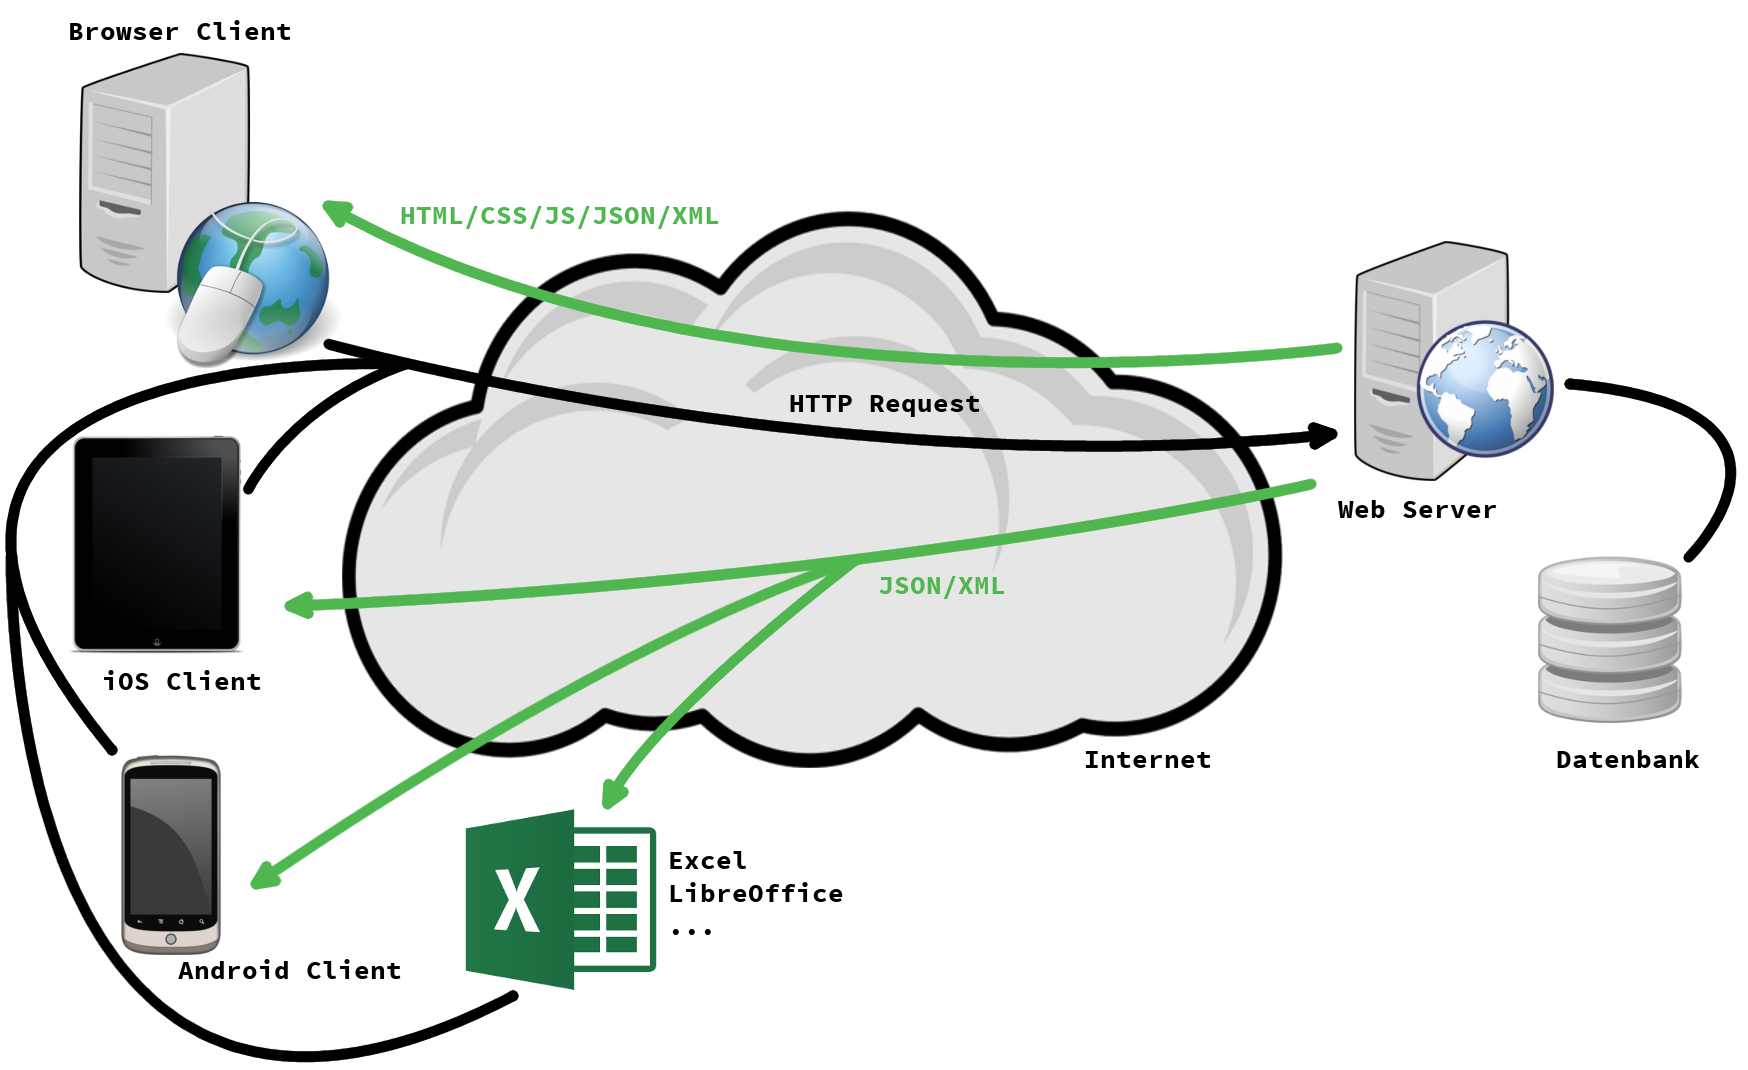
\includegraphics[width=0.6\textwidth]{img/webservice.png}
	\captionsetup{format=hang}
	\caption{Prinzip eines Webservice}
	\small Quelle: \url{https://www.ransoft.at/images/others/webservice.png}
	\label{fig:webservice}
\end{figure}
% !TEX root =  master.tex
\section{\acf{DTO}}
\label{sec:dto}
Das \ac{DTO} ist ein Entwurfsmuster aus dem Bereich der Softwareentwicklung.
Es wird genutzt, um mehrere Objekte in einem Programmaufruf zusammenzufassen, weshalb es Anwendung in verteilten Systemen findet.

Ein \ac{DTO} entspricht eigentlich dem \ac{POJO}.
Es hat nahezu die selben Attribute, kann aber nach Belieben verändert werden.
So kann man sich mittels des \ac{DTO} nur einige Attribute anzeigen lassen und die Entität bleibt unberührt.

Die \acsp{DTO} werden in diesem Projekt dazu genutzt, um die Daten aus der Datenhaltungsschicht der Drei-Schichten-Architektur in die Logik- bzw. Fachkonzeptschicht zu transferieren. Denn eine Entität verlässt niemals die Datenhaltungsschicht.
Von dort aus werden sie an die Benutzerschicht weitergeleitet.

\subsection{Umwandlung der Entität zu und von einem \acf{DTO}}
\label{ssec:umwandlung_dto}
Wie bereits beschrieben kommen in diesem Projekt \acp{DTO} zum Einsatz. Um eine Umwandlung zu realisieren wurden zwei Java-Klassen implementiert: \textit{EntityToToHelper} und \textit{ToToEntityHelper}. \\

Die Klasse \textit{EntityToToHelper} ist dafür verantwortlich, die zuvor über das \acs{DAO} angefragte Entität mit all ihren Attributen in ein \acs{DTO} umzuwandeln, sodass es transferierbar ist. \\
Ein Beispiel für die Umwandlung in ein \acs{DTO} befindet sich im Anhang \vref{lst:EntityToToHelper_movie}. \\
Die Klasse \textit{ToToEntityHelper} ist dafür verantwortlich die zuvor über das \acs{JSON} übermittelte \acs{DTO} mit all seinen Attributen in ein Entität umzuwandeln, sodass es persistier-, änder- oder löschbar ist.\\ 
Ein Beispiel für die Umwandlung in eine Entität befindet sich im Anhang \vref{lst:ToToEntityHelper_movie}.



% !TEX root =  master.tex
\chapter{Front-End}

\section{Technologien}
\label{sec:technologien}

Für das hier erstellte Kinoreservierungsprogramm wurde die Verwendung von Java\footnote{\url{https://java.com/de/download/} -- Version 8.0.141 verwendet} für das Back-End vorgegeben. 

Als Java-\acs{IDE} kommt Eclipse\footnote{\url{https://www.eclipse.org/} -- Version: Photon Release (4.8.0)} zum Einsatz, da es aus vorangegangenen Vorlesungen bekannt ist.
Für die Kommunikation zwischen den einzelnen Schichten der Drei-Schichten-Architektur kommen \acs{REST}ful-Webservices in Verbindung mit Jersey\footnote{\url{https://jersey.github.io/} -- Version 1.19.4} sowie \acp{DTO} zum Einsatz (Kapitel \vref{sec:dto}), die zwischen den einzelnen Schichten transferiert werden.

Um eine Datenhaltung und den Austausch von Informationen zu gewährleisten, wurde sich in dieser Arbeit für eine Postgres Datenbank entschieden.
Der Zugriff auf die Datenbank erfolgt mittels der \ac{JPA} in Verbindung mit EclipseLink (Kapitel \vref{ssec:jpa}).
% !TEX root =  master.tex
\section{Startseite mit Filmübersicht}

Auf der Startseite sieht der Benutzer direkt das Kinoprogramm.
Ganz oben befindet sich ein \enquote{Karussell} mit den aktuellen Blockbustern.
Direkt darunter folgt dann die Liste mit den Filmen.

\begin{figure}[ht]
	\centering
	\subfloat[Desktop-Computer]{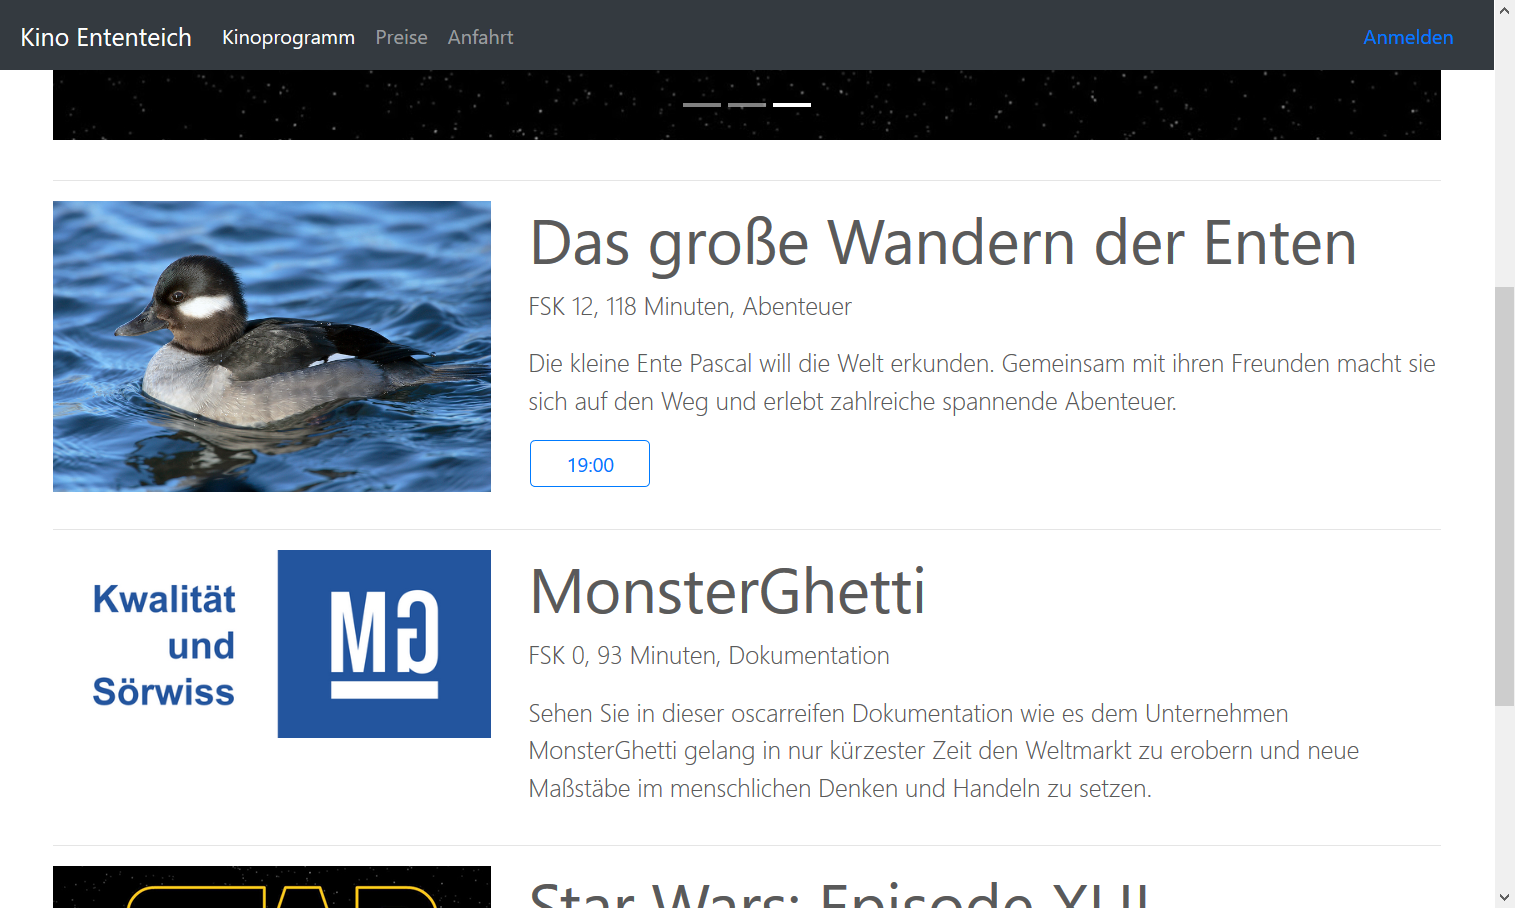
\includegraphics[height=0.28\textheight]{img/screenshots/startseite01}
	\label{fig:startseite01}}
	\hfill
	\subfloat[Mobiles Gerät]{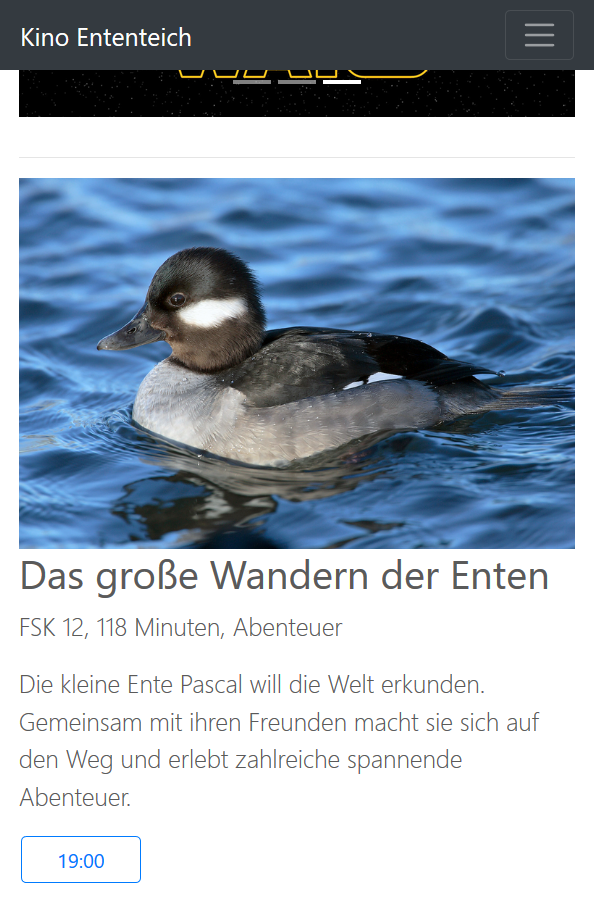
\includegraphics[height=0.28\textheight]{img/screenshots/startseite02}
	\label{fig:startseite02}}
	\caption{Filmübersicht auf der Startseite}
\end{figure}

Dabei ist zu jedem Film neben dem Titel auch noch ein Bild zu sehen.
Allgemeine Informationen zum Film sowie eine Beschreibung ermöglichen es dem Benutzer, sich einen schnellen ersten Eindruck von dem jeweiligen Film zu verschaffen.
Durch Anklicken des Filmtitels oder des Bildes gelangt man zu den Vorstellungen und weiteren Details.
Um Benutzern einen Klick zu ersparen, sieht man sogar direkt die heutigen Vorstellungen und kann gegebenenfalls sofort zu diesen Vorstellungen springen und Sitzplätze auswählen.

Je nach Größe des Bildschirms, wir der Inhalt entsprechend angezeigt.
Bei breiten Bildschirmen, wie es meist bei Desktop-Computern und Laptops der Fall ist, ist genügend Platz, um Bild und Text nebeneinander anzuzeigen.
Bei Smartphones hingegen, wäre das Bild so kaum erkennbar und es würden nicht viele Wörter in eine Zeile passen.
Dementsprechend werden bei solchen Bildschirmen Bild und Text untereinander angezeigt.
All diese Anpassungen werden durch \acs{CSS}-Anweisungen veranlasst, inhaltlich gibt es keine Unterschiede.
% !TEX root =  master.tex
\section{Filmdetails und Vorstellungsauswahl}

Nachdem die Daten wie in Quelltext \ref{lst:load_movie_and_shows} geladen wurden, muss nun das \acs{DOM} entsprechend verändert werden.
Die statische \acs{HTML}-Seite ist dabei auf das Wesentliche reduziert und enthält neben der Menüleiste und der Fußzeile folgenden Teil:

\begin{lstlisting}[style=lstHTML]
<div class="container" id="movie">
	<!-- Informationen zum Film werden hier eingefügt -->
	<table class="table" id="shows">
		<tr>
			<th>Tag</th>
			<th>Vorführungen</th>
		</tr>
		<!-- die einzelnen Vorstellungen werden hier eingefügt -->
	</table>
	<!-- Bewertungen werden hier eingefügt -->
</div>
\end{lstlisting}
\captionof{lstlisting}{\acs{HTML}-Seite für Filmdetails}
\label{lst:html_movie_and_shows}

An den gekennzeichneten Stellen wird später der Inhalt, der aus dem Back-End geladen wurde, eingefügt.
Dafür gibt es kleinere Vorlagen mit Platzhaltern.
In Quelltext \ref{lst:html_template_movie_detail} sieht man die Vorlage für die Filmdetails.

\begin{lstlisting}[style=lstHTML,escapeinside=``]
<div class="row featurette">
	<div class="col-12 col-sm-4">
		<img class="featurette-image img-fluid mx-auto" src="./img/`\textcolor{red}{\{movieID\}}`.jpg" alt="`\textcolor{red}{\{movieTitle\}}`" width="100%">
	</div>
	<div class="col-12 col-sm-8">
		<h2 class="featurette-heading">`\textcolor{red}{\{movieTitle\}}`</h2>
		<p class="lead">FSK `\textcolor{red}{\{movieFSK\}}`, `\textcolor{red}{\{movieDuration\}}` Minuten, `\textcolor{red}{\{movieGenres\}}`</p>
		<p class="lead rating-`\textcolor{red}{\{movieRatingRounded\}}`">`\textcolor{red}{\{movieRating\}}`</p>
	</div>
</div>

<div class="row featurette">
	<div class="col-12">
		<p class="lead">`\textcolor{red}{\{movieDescription\}}`</p>
	</div>
</div>
\end{lstlisting}
\captionof{lstlisting}{\acs{HTML}-Vorlage mit Platzhaltern für Filmdetails}
\label{lst:html_template_movie_detail}

In JavaScript wird diese Vorlage dann mit Inhalten befüllt.
Nachdem die Daten in der Funktion \textit{displayMovieAndShows()} ein wenig verarbeitet wurden, können sie mit JavaScript bzw. jQuery in die Vorlage und danach ins \acs{DOM} eingefügt werden.

\begin{lstlisting}[language=JavaScript]
$("#movie").prepend(templateMovieDetail
	.replace("{movieID}", movie.id)
	.replace(/\{movieTitle\}/g, movie.name)
	.replace("{movieFSK}", movie.fsk)
	.replace("{movieDuration}", movie.duration)
	.replace("{movieGenres}", genres)
	.replace("{movieRatingRounded}", Math.max(0, Math.min(5, Math.round(rating))))
	.replace("{movieRating}", (movie.ratings.length > 0 ? rating.toFixed(1).replace(".",",") : "") + " (" + movie.ratings.length + " Bewertung" + (movie.ratings.length == 1 ? "" : "en") + ")")
	.replace("{movieDescription}", movie.description)
);
\end{lstlisting}
\captionof{lstlisting}{Einfügen der Filmdetails ins \acs{DOM} mit jQuery}
\label{lst:js_write_movie_detail_to_dom}

Genauso wie die Filmdetails werden auch die Vorstellungen und die Bewertungen ins \acs{DOM} eingefügt.

Zusammenfassend heißt das, dass zuerst einmal die statische und weitestgehend leere \acs{HTML}-Seite geladen wird.
Diese wiederum importiert eine JavaScript-Datei, welche beim Laden der Seite einen Aufruf an das Back-End schickt.
Sobald der Server antwortet, wird die Antwort entsprechend verarbeitet und in JavaScript in kleinere Vorlagen eingefügt.
Die mit Inhalten befüllten Vorlagen werden dann mit jQuery ins \acs{DOM} eingefügt, sodass die \acs{HTML}-Seite die gewünschten Inhalte darstellt.
Dies passiert im Idealfall so schnell, dass es für den Benutzer wirkt, als hätte er die Seite \enquote{ganz normal} geladen.

Damit dies reibungslos funktioniert, ist es essentiell, dass sich die Kommunikation mit dem Server auf ein Minimum beschränkt und keine nicht benötigten oder redundanten Daten transferiert werden.
So ist es zum Beispiel schlecht für die Performance, wenn man im Front-End lediglich eine Liste mit allen Filmen sehen will, aber vom Back-End zu jedem Film alle Vorstellungen mit allen Sitzplätzen erhält.

Genauso muss natürlich die Verarbeitung im Front-End effizient erfolgen.
% !TEX root =  master.tex
\section{Anbindung an das Back-End}
\label{sec:anbindung_backend}

Um die Daten aus der Datenbank bzw. dem Back-End anzuzeigen, werden diese durch einen oder mehrere \acs{AJAX}-Aufrufe nachgeladen.
Beim Laden der Startseite wird die Funktion \textit{loadMovies()} aufgerufen.
Diese wiederum ist nur für die Zuordnung von einem Pfad bzw. einer \acs{URI} zu einer Funktion, die das Ergebnis verarbeitet, da.
Sie würde auch \acs{URL}-Parameter auslesen und in den Aufruf mit einarbeiten, dies ist aber auf der Startseite noch nicht notwendig.

\begin{lstlisting}[language=JavaScript]
const URL_SERVER = "http://localhost:8080/cinema-system";
const PATH_ALL_MOVIES = "/movie/getAllMovies";

function getData (path, func) {
	$.ajax({
		type: "GET",
		url: URL_SERVER + path,
		success: (data) => func(data),
		error: function (xhr,status,error){
			console.log(xhr, status, error);
			func([]);
		}
	});
}

function loadMovies () {
	getData(PATH_ALL_MOVIES, displayMovies);
}

function displayMovies (movies) {
	...
}
\end{lstlisting}
\captionof{lstlisting}{\acs{AJAX}-Aufruf, um alle Filme zu erhalten}
\label{lst:ajax_all_movies}
% !TEX root =  master.tex
\section{Implementierung des Saalplans}
\authorsection{\authorNL}

\subsection{Darstellung des Kinosaals}

Eine zentrale Aufgabe im Front-End war es, den Kinosaal mit den Sitzen anzuzeigen und dem Benutzer zu ermöglichen, Plätze auszuwählen.

Dies lässt sich mit einfachen Mitteln auch in \acs{HTML} umsetzen, z.B. mit \textit{div}-Elementen, bei denen man Größe und Farbe festlegt.
Mit JavaScript wird dann implementiert, was passiert wenn ein Sitzplatz angeklickt wird.

\begin{figure}[ht]
	\centering
	\subfloat{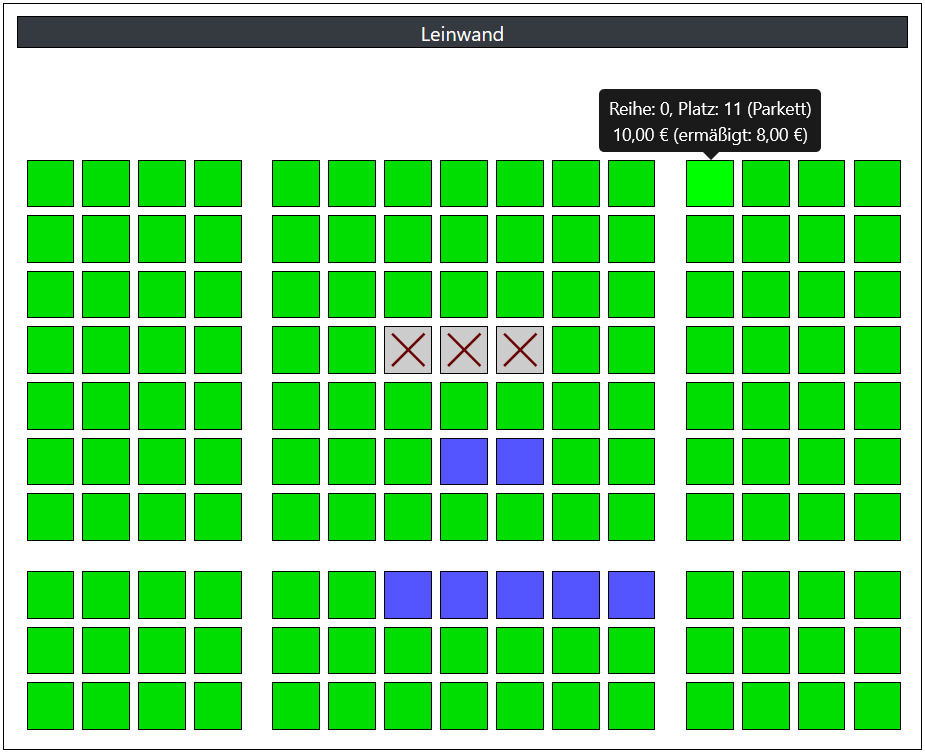
\includegraphics[height=0.295\textheight]{img/screenshots/saalplan01}}
	\hfill
	\subfloat{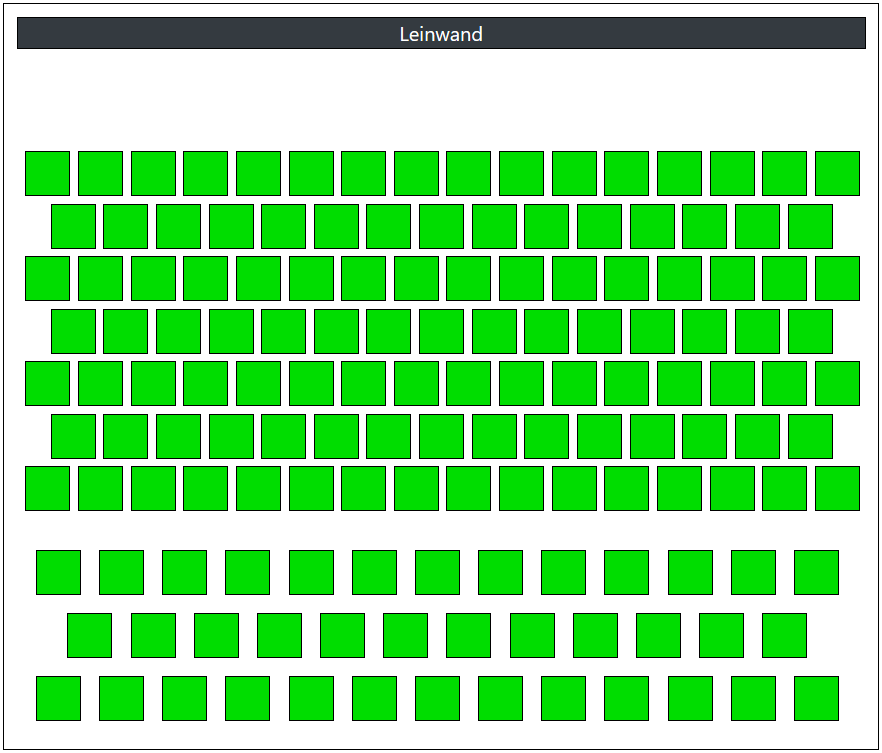
\includegraphics[height=0.295\textheight]{img/screenshots/saalplan03}}

	\caption{Saalpläne}
	\label{fig:saalplan}
\end{figure}

In Abbildung \vref{fig:saalplan} kann man sehen, wie der Kinosaal im Browser dargestellt wird.
Eine Box außen bildet die Umrandung und stellt den Saal dar.
Darin befindet sich eine zweite farblich hervorgehobene Box, die die Leinwand abbildet, damit die Benutzer wissen, wo im Kinosaal vorne und hinten ist, und sie somit ihre Entscheidung, wo sie sitzen möchten, treffen können.
Darunter finden sich dann die Sitzplätze.

Die Sitzplätze sind dabei farblich gekennzeichnet, um anzuzeigen, ob ein Sitzplatz frei oder belegt ist.
Belegte Sitze sind einerseits grau, andererseits auch noch mit einem Kreuz versehen, um Menschen, die in ihrer Farbwahrnehmung eingeschränkt sind, zu berücksichtigen.
Außerdem werden ausgewählte Sitze blau markiert und der Sitz, über dem aktuell die Maus ist, wird ebenso hervorgehoben.
Ein Tooltip mit einer kurzen Beschreibung und Details zu Kategorie und Preis, gibt dem Benutzer weitere Informationen.

Das Aussehen der Sitzplätze wird über Klassen und eine eigene \acs{CSS}-Datei definiert, sodass sich dies schnell anpassen lässt und zum Beispiel die Farbe der Sitzplätze mit einem Mal änderbar ist.

\begin{figure}[ht]
	\centering
	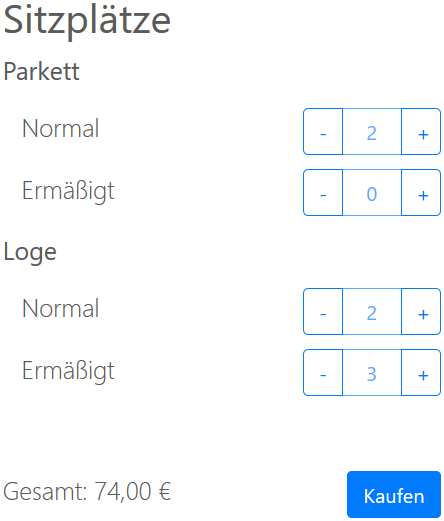
\includegraphics[width=0.4\textwidth]{img/screenshots/saalplan02}
	\captionsetup{format=hang}
	\caption{Preisstufen}
	\label{fig:saalplan02}
\end{figure}

Wählt man nun Sitzplätze aus, so muss man noch angeben, wie viele Tickets zum normalen Preis man kaufen möchte und wie viele zu einem ermäßigten Preis.
Daraus wird dann direkt der Preis berechnet und angezeigt (siehe Abbildung \ref{fig:saalplan02}).
Je nach Bildschirmgröße und -dimensionen werden diese Element neben dem Saalplan oder darunter angezeigt.
Mit dem \enquote{Kaufen}-Button gelangt man dann zur nächsten Seite, um weitere Daten anzugeben.

In der ersten Implementierung wurden der Saal und die Sitzplätze mit absoluten Größenangaben definiert.
So hatte das \textit{div}-Element, das einen Sitzplatz darstellt, als Höhe und Breite \textit{20px} gesetzt und eine Position relativ zur links oberen Ecke des Saals in Pixeln angegeben.
Die Koordinaten kommen dabei direkt aus dem Back-End bzw. der Datenbank.
Dies ermöglicht es, nicht nur einfach alle Plätze nebeneinander anzuzeigen, sondern auch Gänge einzufügen, Plätze versetzt anzuordnen, die Abstände zwischen den Sitzen individuell zu gestalten und somit den Saalplan an die Realität anzupassen.

Durch die Verwendung absoluter Größen in Pixeln, ist jedoch das Benutzererlebnis auf kleinen Bildschirmen schlechter.
Der Saal ist erst einmal breiter als der Bildschirm und der Benutzer muss herauszoomen und die Größe selbst anpassen.
Das Gleiche gilt für Benutzer eines Desktop-Computers, wenn sie die Fenstergröße anpassen.

Um dies zu verbessern, wird beim erstmaligen Laden sowie bei jeder Änderung der Fenstergröße, die Größe des Saals und der Sitzplätze neu berechnet.
Die Größenangaben aus der Datenbank werden dabei genutzt und entsprechend skaliert, sodass der Saalplan weder die volle Breite, noch die volle Höhe des Bildschirms überschreitet.
Um den Berechnungsaufwand zu reduzieren, sind die Koordinaten aller Sitzplätze prozentual angegeben.
Diese prozentualen Angaben beziehen sich dabei auf den \textit{div}-Container, der den Saal darstellt.
Dementsprechend muss lediglich die Größe des Saals und die Größe der Sitzplätze berechnet werden.

Ein Sitzplatz wird durch eine \acs{HTML}-Vorlage erstellt.
Die aus der Datenbank stammenden und in JavaScript verarbeiteten Werte werden zunächst in die Vorlage und im Anschluss ins \acs{DOM} eingefügt.

\begin{lstlisting}[style=lstHTML, caption={\acs{HTML}-Vorlage für die Darstellung eines Sitzplatzes}, label={lst:html_template_seat}]
<div id='`\textcolor{red}{\{seatID\}}`'
	class='seat `\textcolor{red}{\{classes\}}`'
	style='left: `\textcolor{red}{\{posx\}}`%; top: `\textcolor{red}{\{posy\}}`%;'
	title='`\textcolor{red}{\{tooltip\}}`'>
</div>
\end{lstlisting}

Die Gestaltung erfolgt dabei vollkommen über \acs{CSS}-Klassen, die in JavaScript hinzugefügt oder entfernt werden.

\begin{lstlisting}[style=lstCSS, caption={Optische Gestaltung der Sitzplätze}, label={lst:css_seat}]
.seat {
	border: 1px solid black;
}
.available {
	background-color: #0d0;
}
.occupied {
	background-color: #ccc;
}
.hovering {
	background-color: #0f0;
}
.selected {
	background-color: #55f;
}
\end{lstlisting}

\subsection{Reaktion auf Benutzerinteraktion}

Sobald der Benutzer einen Sitzplatz anklickt, wird diese Information an die zugehörige Funktion weitergereicht.

\begin{lstlisting}[language=JavaScript, caption={Erkennen des Anklickens eines Sitzplatzes}, label={lst:js_onclick}]
$(".seat").on("click", function () {
	var seatId = $(this).attr("id");
	if (seatId in selection) {
		removeSeatFromSelection(seatId, this);
	}
	else {
		addSeatToSelection(seatId, this);
	}
});
\end{lstlisting}

Wenn der Benutzer einen Sitzplatz auswählen möchte, muss noch einmal überprüft werden, ob dieser auch wirklich noch frei ist.
Zusätzlich soll der Sitzplatz für den Benutzer vorgemerkt werden, damit in der Zwischenzeit kein anderer den Sitzplatz reserviert.

Dafür wird eine \acs{AJAX}-Anfrage an das Back-End gesendet.
Dabei wird einerseits die Vorstellung und der ausgewählt Sitzplatz mitgegeben, andererseits aber auch eine Benutzeridentifizierung in Form einer zufälligen Zeichenkette, die im Browser des Benutzers als Cookie gespeichert wird.

\begin{lstlisting}[language=JavaScript, caption={Senden einer Anfrage, den Sitzplatz zu blocken}, label={lst:js_ajax_send_block}]
function addSeatToSelection (seatId, seatObj) {
	// prepare data for ajax
	var block = {show: {id: urlparameters.get("id")},
		seat: {id: seatId},
		sessiontoken: cookie};

	// send ajax
	var data = "block=" + JSON.stringify(block);
	$.ajax({
		type: "POST",
		url: "http://localhost:8080/cinema-system/reservation/block",
		data: data,
		contentType: "application/json; charset=utf-8",
		success: (data) => processBlockingResult(data, seatId, seatObj),
		error: function (xhr,status,error){
			console.log(xhr, status, error);
			processBlockingResult(null, seatId, seatObj);
		}
	});
}
\end{lstlisting}

Die Antwort des Servers wird an die entsprechende Funktion weitergegeben.
Dort wird nun überprüft, ob das Blocken des Sitzplatzes erfolgreich war oder nicht.

\begin{lstlisting}[language=JavaScript, caption={Verarbeiten der Server-Antwort beim Versuch, einen Platz zu blocken}, label={lst:js_ajax_process_block}]
function processBlockingResult (data, seatId, seatObj) {
	if(data != null) {
		var seatIdResponse = data.seat.id;
		seats[seatId].isBlocked = false;
		$(seatObj).addClass("selected available");
		$(seatObj).removeClass("occupied");
		selection[seatIdResponse] = true;
		numberOfTickets[getCategoryOfSeat(seatIdResponse)] += 1;
		updatePriceBox();
	} else {
		seats[seatId].isBlocked = true;
		$(seatObj).removeClass("available hovering");
		$(seatObj).addClass("occupied");
	}
}
\end{lstlisting}

Zum einen werden alle nötigen Variablen aktualisiert, zum anderen wird die Benutzeroberfläche entsprechend angepasst.
Dies umfasst den angeklickten Sitz selbst und auch die in Abbildung \vref{fig:saalplan02} gezeigten Auswahlmöglichkeiten für die Ermäßigung und Preisstufen der Sitzplätze.


% bibliography
\printbibliography[title=Literaturverzeichnis]
\cleardoublepage

% appendix
\appendix
\ihead{\appendixname~\thechapter}

\chapter{Abbildungen}
\begin{sidewaysfigure}
	\centering 
	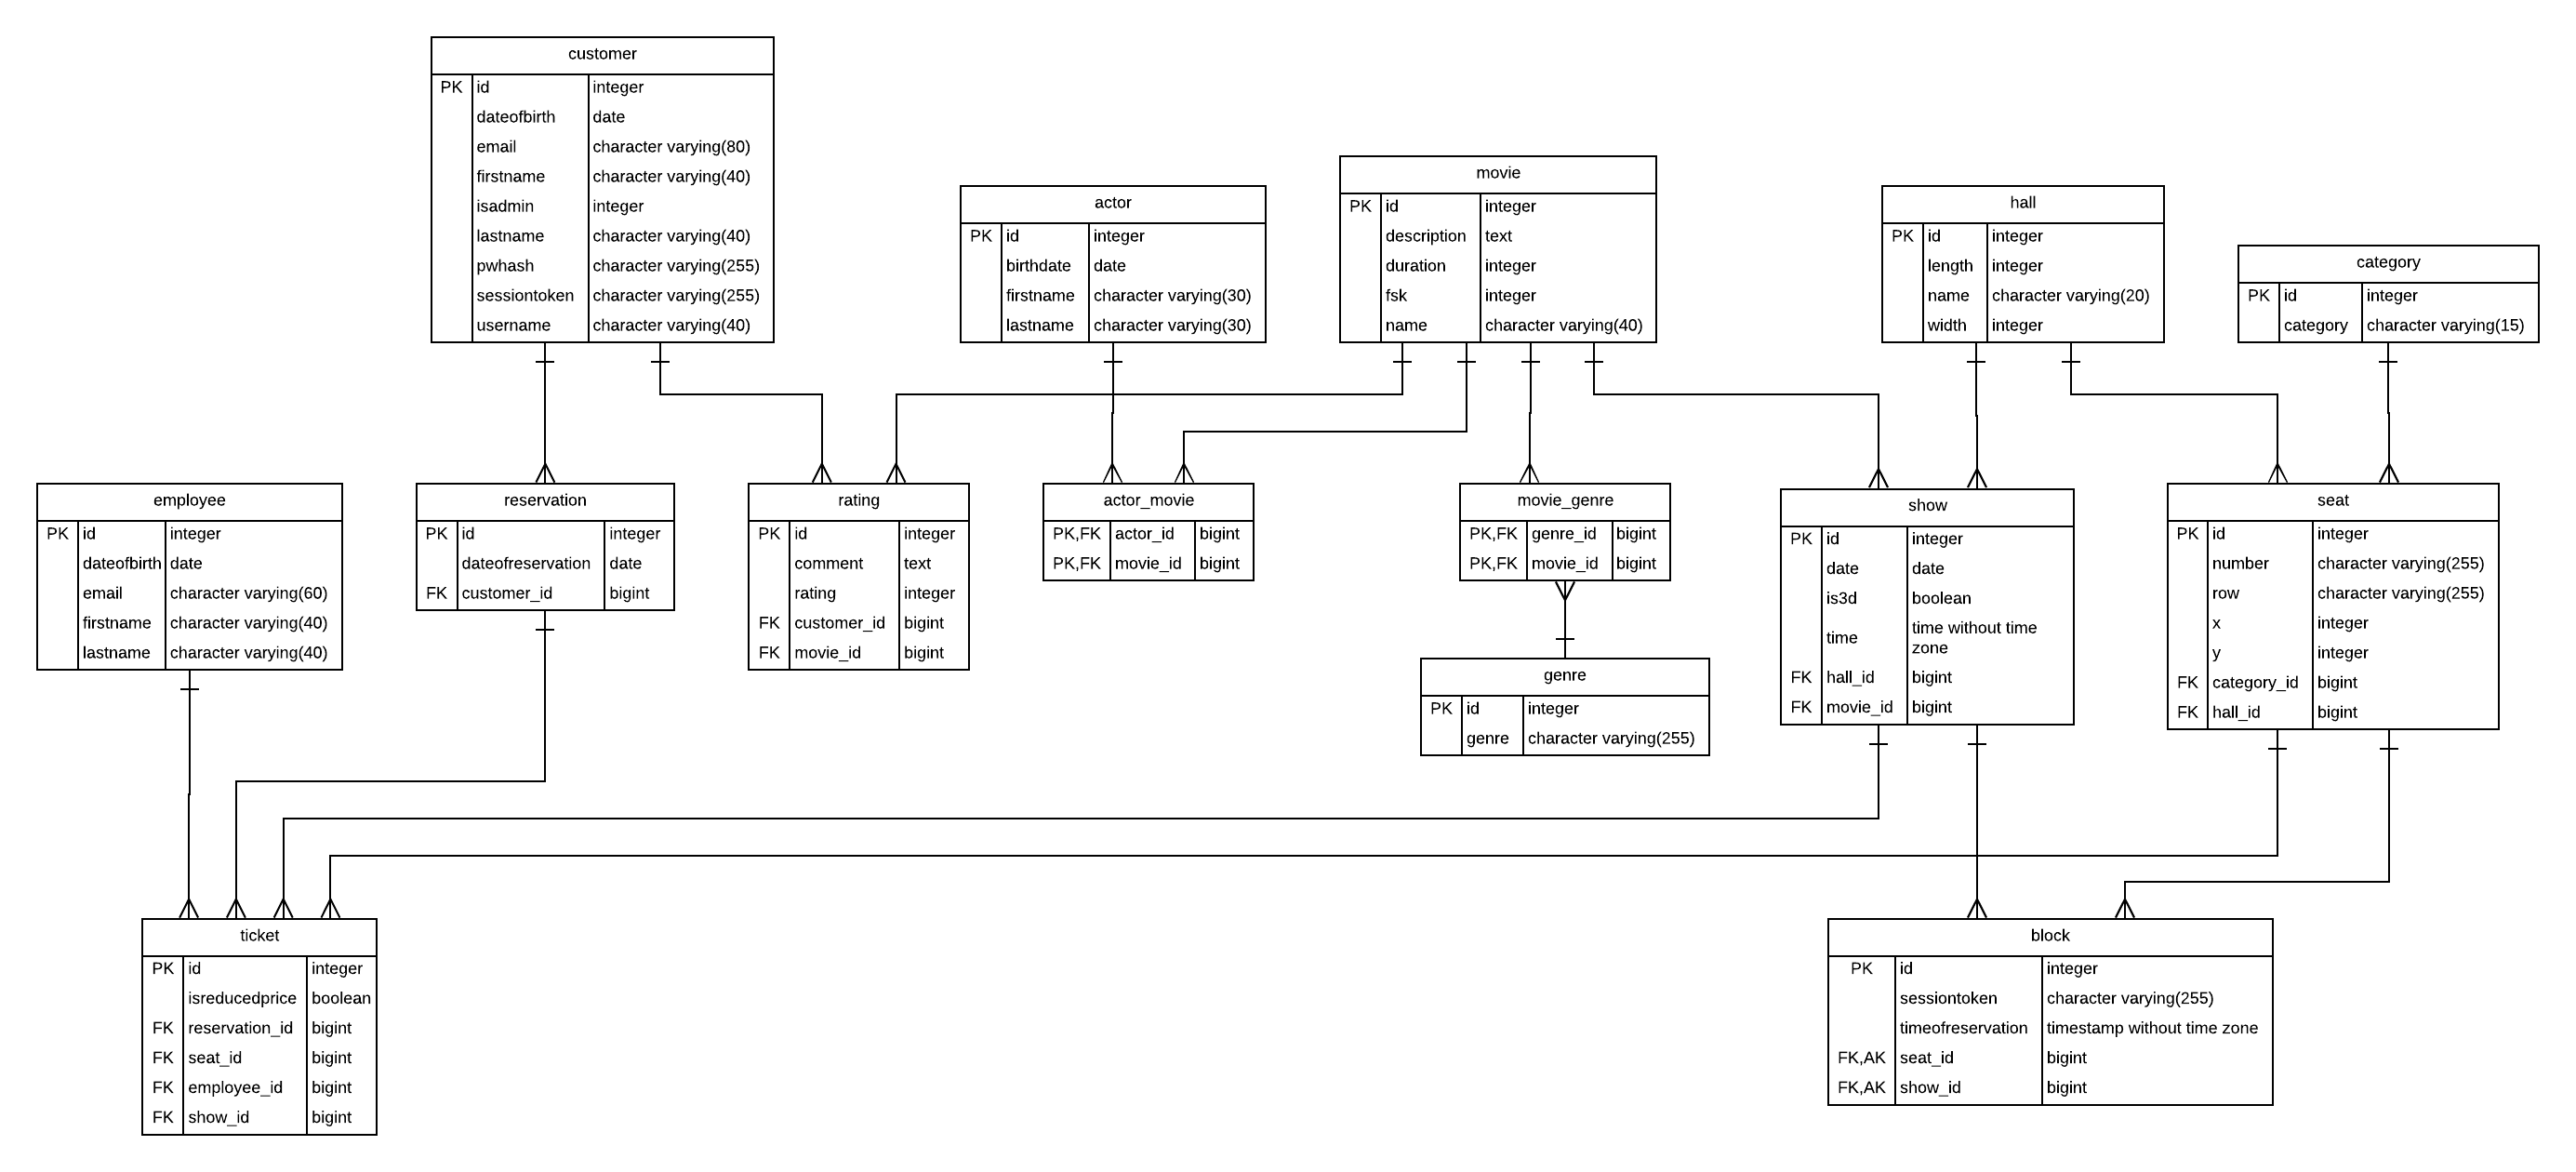
\includegraphics[keepaspectratio, width=1.0\textwidth, height=1.0\textheight]{img/ER-Modell}
	\captionsetup{format=hang}
	\caption{\acs{ER-Modell} der Datenbank}
	\small Quelle: eigene Darstellung mittels \url{https://www.lucidchart.com/}
	\label{fig:Anhang_ER-Modell}
\end{sidewaysfigure}

\chapter{Quellcode}
\begin{minipage}{\linewidth}
	\begin{lstlisting}[style=lstJava]
	public static MovieTo createMovieTo ( Movie entity, boolean withShow )
	{
	if ( null != entity )
	{
	MovieTo movieTo = new MovieTo();
	movieTo.setId(entity.getId());
	movieTo.setDescription(entity.getDescription());
	movieTo.setFsk(entity.getFsk());
	movieTo.setDuration(entity.getDuration());
	movieTo.setName(entity.getName());
	movieTo.setGenres(createGenreTos(entity.getGenres()));
	movieTo.setRatings(createRatingTos(entity.getRatings()));
	if ( withShow )
	{
	movieTo.setShows(createShowTos(entity.getShows(), false));
	} // end withSow
	movieTo.setActors(createActorTos(entity.getActors()));
	return movieTo;
	}  // end if null
	return null;
	}
	\end{lstlisting}
	\captionof{lstlisting}{Erstellen eines Movie-\acs{DTO} aus einer Movie-Entität mit Hilfe des eigen erstellten EntityToToHelper}
	\label{lst:EntityToToHelper_movie}
\end{minipage}

\begin{minipage}{\linewidth}
	\begin{lstlisting}[style=lstJava]
	public static Movie createMovieEntity ( MovieTo transferObject, boolean withShow )
	{
		if ( null != transferObject )
		{
			Movie movie = new Movie();
			movie.setId(transferObject.getId());
			movie.setActors(createActorEntities(transferObject.getActors()));
			movie.setDescription(transferObject.getDescription());
			movie.setFsk(transferObject.getFsk());
			movie.setDuration(transferObject.getDuration());
			movie.setName(transferObject.getName());
			movie.setRatings(createRatingEntities(transferObject.getRatings()));
			if ( withShow )
			{
				movie.setShows(createShowEntities(transferObject.getShows(), false));
			}
			movie.setGenres(createGenreEntities(transferObject.getGenres()));
			return movie;
		}
		return null;
	}
	\end{lstlisting}
	\captionof{lstlisting}{Erstellen einer Movie-Entität aus einem Movie-\acs{DTO} mit Hilfe des eigen erstellten ToToEntityHelper}
	\label{lst:ToToEntityHelper_movie}
\end{minipage}

% ewerkl.tex
% !TEX root =  master.tex

\clearpage
\chapter*{Ehrenwörtliche Erklärung}

Wir versichern hiermit, dass wir die vorliegende Arbeit
 mit dem Thema: \textit{\DerTitelDerArbeit} selbstständig verfasst und keine anderen als die angegebenen Quellen und
Hilfsmittel benutzt haben. Wir versichern zudem,
dass die eingereichte elektronische Fassung mit der gedruckten Fassung übereinstimmt.

\vspace{2cm}
Ort, Datum

\vspace{5mm}
\authorSG
\hfill \authorRF
\hfill \authorGP

\vspace{5mm}
\hfill \authorRF
\hfill \authorNL
\hfill

\end{document}
